\chapter{Criticalité absorbante et interactions à longue portée en matière molle}

\label{chapter:introduction}

\subparagraph{}Dans cette thèse, nous présentons l'étude comparée de deux phénomènes de matière molle : la transition de réversibilité dans les suspensions cisaillées cycliquement et la transition vers l'écoulement des fluides à seuil. Le but de ce chapitre est d'introduire ces deux phénomènes que rien ne rassemble au premier regard et de motiver leur étude comparée comme des transitions de phase absorbantes.

\subparagraph{}Pour ce faire, nous commencerons par présenter succinctement la phénoménologie de ces transitions, mettant en évidence un comportement singulier et des mécanismes communs. Cette première familiarisation nous amènera alors naturellement à un cadre commun pour l'étude de ces deux phénomènes : celui des transitions de phase absorbantes. Nous proposerons alors de prendre un peu de recul en présentant la phénoménologie globale de ces transitions, analogue à celle des phénomènes critiques d'équilibre. Après une description complète de la classe d'universalité de la percolation dirigée conservée, nous montrerons en quoi la transition de réversibilité et la transition vers l'écoulement en représentent des bons candidats. En accord avec les études précédentes de ces deux systèmes, nous montrerons que leur comportement critique s'éloigne fortement de ce cadre théorique et en proposerons une explication via la nature fondamentalement différente des interactions à longue portée présentes dans ces systèmes. Enfin, nous formulerons les problématiques relatives à ce comportement singulier qui guideront notre étude tout au long de cet ouvrage.

\section{Écoulement des fluides à seuil et cisaillement cyclique des suspensions}

\subparagraph{}Dans cette section, nous présentons succinctement et successivement la transition de réversibilité dans les suspensions cisaillées cycliquement et la transition vers l'écoulement des fluides à seuil. Le rapprochement des deux phénoménologies associées nous permettra alors de comprendre en quoi l'étude comparée de ces deux systèmes représente un objet riche et intéressant.

\subsection{Transition de réversibilité dans les suspensions cisaillées cycliquement}

\subparagraph{}Certains systèmes en matière molle présentent un phénomène intriguant sous l'action d'un cisaillement cyclique. Sous une amplitude de déformation relativement faible, ceux-ci finissent par opérer une dynamique réversible à temps long, laissant le système inchangé d'un cycle de déformation à l'autre. Toutefois, si cette amplitude devient suffisamment grande, le système est soumis à des changements irréversibles en permanence, menant à une évolution constante de sa structure au fil des cycles \cite{eckstein_self_diffusion_1977, breedveld_shear_induced_2001, drazer_microstructure_2004}. Nous appellerons transition de réversibilité le passage d'une phase à l'autre de ce système.

\begin{figure}[h]
	\centering
	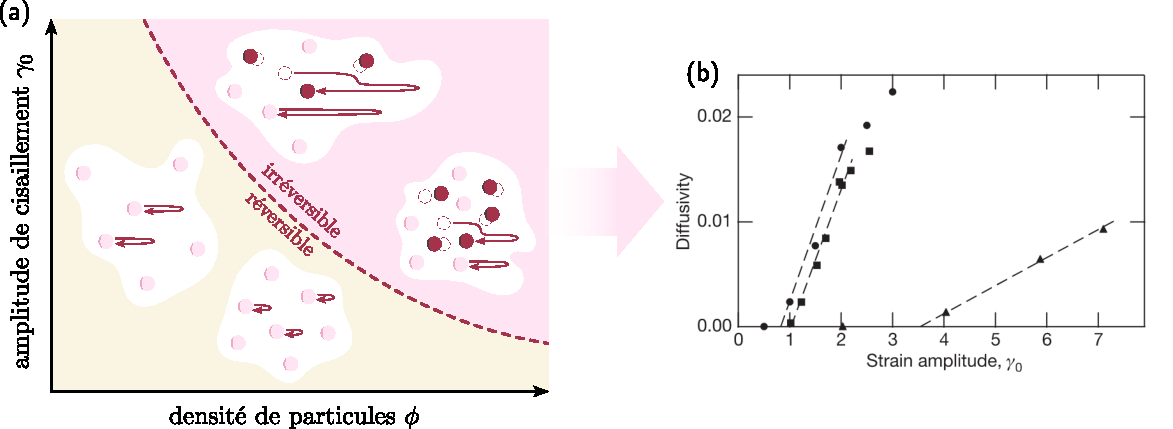
\includegraphics[width=\textwidth]{Chapitre1/Figures/Chapo/suspensions.pdf}
	\caption{(a) Diagramme de phase de la transition de réversibilité inspiré de \cite{maegochi_critical_2021}. Les particules rouges montrent une dynamique irréversible. (b) Évolution du coefficient de diffusion stroboscopique en fonction de l'amplitude de cisaillement dans les expériences de Pine et al. \cite{pine_chaos_2005}}
	\label{fig:suspchapo}
\end{figure}

\subparagraph{}La transition de réversibilité peut être illustrée parfaitement par les expériences menées par Pine et al. \cite{pine_chaos_2005}, dans lesquelles une suspension peu dense est cisaillée dans un écoulement de Couette cylindrique. En suivant l'évolution de la position des particules du système d'un cycle à l'autre, les auteurs ont pu observer deux comportements distincts. Pour une amplitude de cisaillement suffisamment faible $\gamma_0 < \gamma_{0,c}$, les particules conservent la même position d'un cycle à l'autre. Cependant pour $\gamma_0 > \gamma_{0,c}$, les particules se déplacent entre le début et la fin d'un cycle. En étudiant la dynamique stroboscopique du système, i.e. à chaque début de cycle, la suspension est donc immobile pour $\gamma_0 < \gamma_{0,c}$ et elle diffuse pour $\gamma_0 > \gamma_{0,c}$. Il est alors possible de visualiser cette transition en représentant l'évolution du coefficient de diffusion stroboscopique $D_0$ associé en fonction de l'amplitude de cisaillement $\gamma_0$, comme sur la \autoref{fig:suspchapo}-(b).

\subparagraph{}L'origine de cette diffusion stroboscopique à l'échelle macroscopique est attribuée à des interactions microscopiques irréversibles entre les particules, comme illustré sur la \autoref{fig:suspchapo}-(a). Lorsque les particules sont suffisamment éloignées au cours du cisaillement, leur dynamique est uniquement régie par les équations de Stokes, qui ont la propriété d'être réversibles dans le temps. D'un cycle à l'autre, la dynamique est donc identique. Toutefois, lorsque celles-ci sont suffisamment rapprochées par le cisaillement (ou proches initialement du fait d'une forte densité), elles interagissent entre elles au cours du cycle via des interactions locales irréversibles (contacts), induisant de ce fait une évolution d'un cycle à l'autre. C'est la succession de ces interactions irréversibles qui induit une diffusion stroboscopique sous grande amplitude de cisaillement \cite{corte_random_2008}.

\subsection{Transition vers l'écoulement des fluides à seuil}

\subparagraph{}Le second phénomène auquel nous nous intéressons est l'écoulement des fluides à seuil. Les fluides à seuil représentent des objets peuplant notre quotidien à différentes échelles. Nous les retrouvons à l'état naturel par l'écume marine ou les argiles mais aussi par les matériaux d'origine anthropique comme le dentifrice ou la mayonnaise. Leur particularité vient de leurs propriétés rhéologiques, bien plus complexes que celles des fluides newtoniens comme l'eau ou le miel.

\begin{figure}[h]
	\centering
	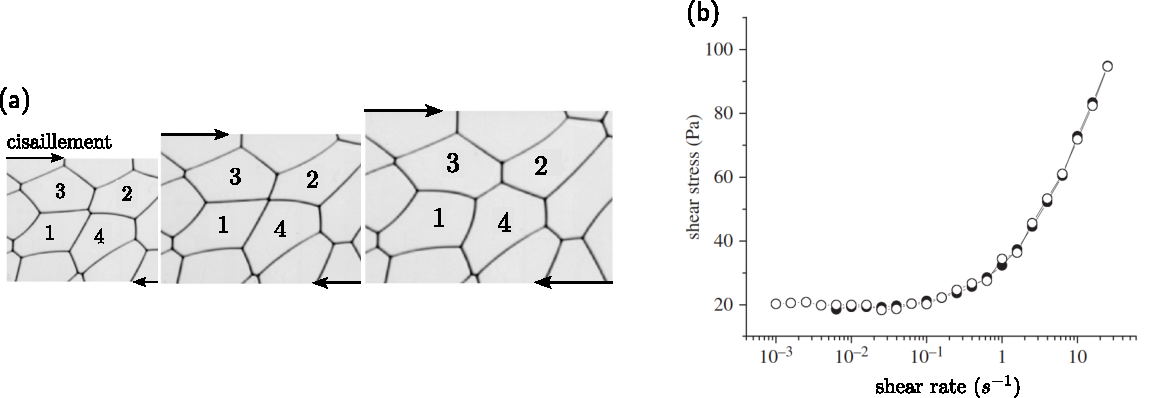
\includegraphics[width=\textwidth]{Chapitre1/Figures/Chapo/yielding.pdf}
	\caption{(a) Image tirée de \cite{dollet_rheology_2014} d'un réarrangement plastique dans une mousse : les bulles voisines changent leur contact afin de minimiser la contrainte supportée. (b) Evolution de la contrainte de cisaillement en fonction du taux de cisaillement appliqué. Données tirées de \cite{moller_origin_2009}}
	\label{fig:yieldingchapo}
\end{figure}


\subparagraph{}Si l'on considère le cas du cisaillement simple  d'un tel fluide, celui-ci possède la spécificité de ne s'écouler que si la contrainte de cisaillement $\Sigma$ appliquée est supérieure à une certaine contrainte seuil $\Sigma_c$ propre au matériau \cite{bonn_yield_2017, nicolas_deformation_2018}. Un exemple édifiant est celui du dentifrice, qui ne s'écoule de son tube que lorsqu'on le presse suffisamment. 

\subparagraph{}En-deçà de la contrainte seuil, après un éventuel régime transitoire, le matériau répond élastiquement à la sollicitation à l'échelle locale comme globale, définissant un taux de cisaillement nul $\dot{\gamma}=0$ dans l'état stationnaire. En revanche, au-delà de cette contrainte seuil, l'état stationnaire du système est caractérisé par la présence continue de réarrangements plastiques locaux (voir \autoref{fig:yieldingchapo}-(a)) \cite{princen_rheology_1986, biance_topological_2009,picard_elastic_2004}. Pour $\Sigma > \Sigma_c$ la succession de ces évènements résulte alors en un écoulement global et donc un taux de cisaillement moyen non-nul $\dot{\gamma}>0$. Il est ainsi possible de visualiser cette transition en représentant l'évolution du taux de cisaillement moyen en fonction de la contrainte appliquée, comme sur l'exemple de la \autoref{fig:yieldingchapo}-(b).


\subsection{Des similarités non-conventionnelles}

\subparagraph{}Ces phénomènes ont en première apparence très peu de points communs. Toutefois, il existe entre eux des similitudes très fortes, illustrées sur la \autoref{fig:banger}. Tout d'abord, comme lae lecteurice l'aura peut-être déjà remarqué, ceux-ci séparent dans chacun des systèmes concernés deux états : un état actif et un état arrêté. Dans le cas de la transition vers l'écoulement l'état actif correspond à un état fluide tandis que dans la transition de réversibilité il correspond à un état diffusant. Par ailleurs, dans les deux cas, ces états actifs sont composés d'une succession d'évènements locaux. Dans le cas de la transition vers l'écoulement ceux-ci sont représentés par les réarrangements plastiques alors que dans le cas de la transition de réversibilité ce sont les interactions de contact irréversibles.

\begin{figure}[H]
	\centering
	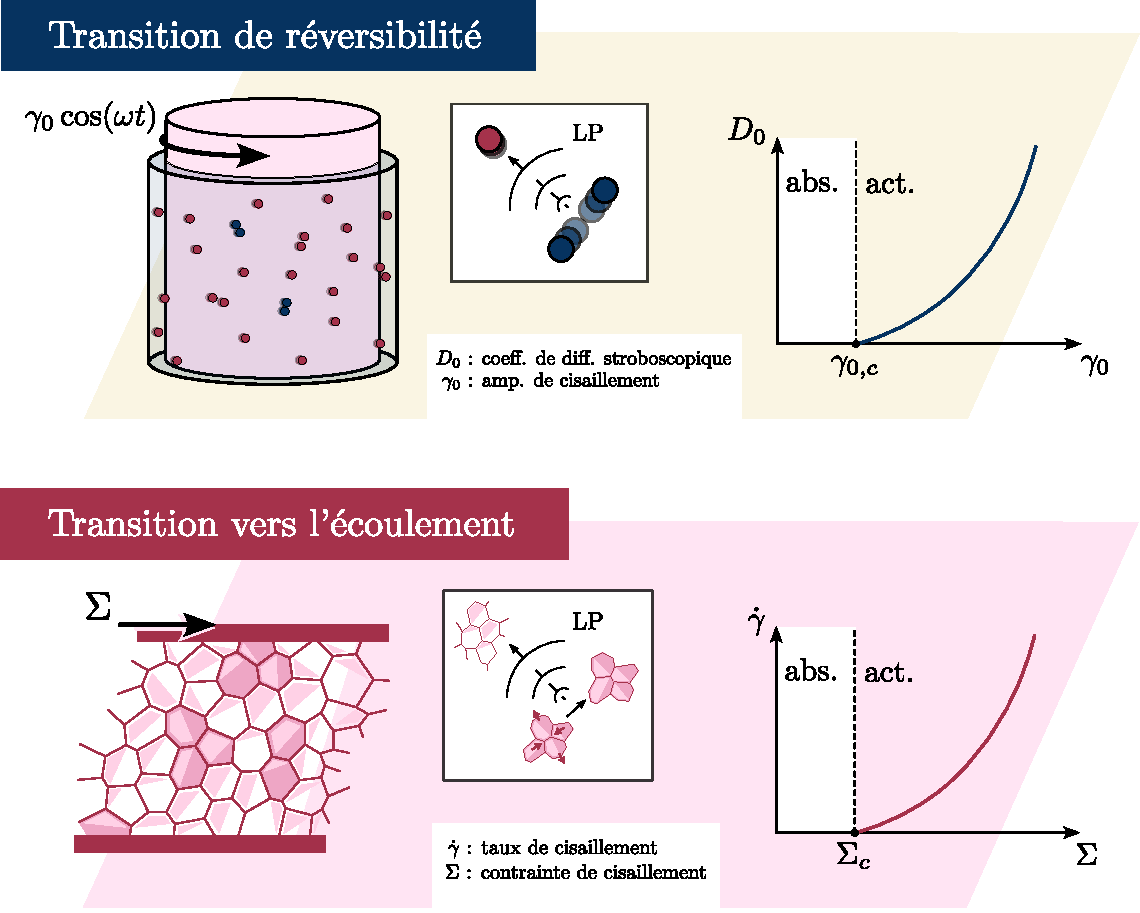
\includegraphics[width=\textwidth]{Chapitre1/Figures/Chapo/Resume.pdf}
	\caption{Illustration schématique du parallèle existant entre la transition de réversibilité dans les suspensions cisaillées cycliquement et la transition vers l'écoulement des matériaux amorphes. LP signifie \textit{longue portée}, abs. signifie \textit{absorbant} et act. signifie \textit{actif}.}
	\label{fig:banger}
\end{figure}

\subparagraph{}De plus, un autre point commun que l'on mettra en évidence dans la suite de ce chapitre est la présence de longue portée. En effet, si dans chacun de ces systèmes la phase active est représentée par des mouvements locaux, il y a de fortes raisons de penser que ceux-ci affectent la dynamique globale via des interactions à longue portée. Dans le cas de la transition de réversibilité dans les suspensions, les particules sont immergées dans un fluide visqueux. Celui-ci est alors capable de propager l'irréversibilité locale à grande distance selon les lois de l'hydrodynamique, affectant de ce fait la dynamique des particules n'interagissant pas directement avec les autres. Dans le cas de la transition vers l'écoulement, les réarrangements plastiques se font dans une matrice élastique. Cette situation largement étudiée montre que ces évènements locaux induisent des interactions à longue portée dans le matériau, susceptibles d'induire d'autres évènements à grande distance. Dans cette optique, la transition vers l'écoulement et la transition de réversibilité peuvent donc être toutes les deux comprises comme des \textbf{transitions de phase absorbantes en présence d'interactions à longue portée}.

\subparagraph{}Enfin, une similarité plus remarquable motive réellement l'étude conjointe de ces deux phénomènes. Celle-ci se rapporte à leur manière d'approcher la phase absorbante. D'une part, dans le cas de la transition vers l'écoulement, les expériences en laboratoire comme les modélisations numériques ont permis de caractériser l'évolution du taux de cisaillement avec la contrainte, montrant une évolution convexe de la courbe descriptive $\dot{\gamma} = f(\Sigma)$. D'autre part, dans le cas de la transition de réversibilité, une modélisation numérique simple faisant intervenir les interactions à longue portée a de la même façon montré une évolution convexe du coefficient de diffusion stroboscopique avec le paramètre de transition \cite{mari_absorbing_2022}. Ce point commun se révèle alors très surprenant puisque, comme nous le montrerons dans la suite, le cadre théorique générique pour ces transitions avec interactions à longue portée ne permet pas d'expliquer une telle convexité, atypique dans le domaine des phénomènes critiques. 

\subparagraph{}Dans ce chapitre, nous proposons de préciser les similitudes entre ces deux phénomènes et de développer cette confrontation théorique afin de pouvoir finalement la problématiser. Pour ce faire, nous commencerons par introduire la notion de transition de phase absorbante dans la théorie des phénomènes critiques. Nous décrirons ensuite la classe d'universalité de la percolation dirigée conservée, a priori la plus à même de décrire ces deux phénomènes. Puis, par sa généralisation à longue portée, nous montrerons en quoi la convexité observée dans ces deux transitions les exclue de ce cadre. Enfin, nous soulignerons les ingrédients physiques précis qui suggèrent la compréhension de la spécificité de ces phénomènes via une approche commune.

\section{Transitions de phases absorbantes}

\subparagraph{}Dans cette section, nous présentons dans un premier temps la phénoménologie des phénomènes critiques à l'équilibre. La présentation des théories et des concepts sous-jacents à ces phénomènes largement étudiés nous permettra de mieux appréhender la seconde partie de cette section. Dans celle-ci, nous introduirons par analogie la notion de transition de phase absorbante et les spécificités qui lui sont associées. Cette partie nous permettra alors de constituer une première boîte à outils incontournable pour l'étude des transitions de réversibilité et d'écoulement.

\subsection{Phénomènes critiques à l'équilibre}

\subsubsection{Phénoménologie d'une transition de phase}

\subparagraph{}La plupart des systèmes physiques existent sous plusieurs états possibles. Par exemple, nous connaissons l'eau, indispensable à la vie sur Terre, sous différentes formes. Elle peut se faire vapeur dans l'atmosphère, liquide dans les rivières ou bien encore solide sur les glaciers. Ces différents états possibles, appelés plus généralement phases du système, présentent des domaines de stabilité qui dépendent de paramètres extérieurs. Par exemple, dans le cas de l'eau, la phase stable dépend de la température et de la pression dans l'environnement considéré. En variant ces paramètres, il est possible de passer d'un domaine de stabilité à un autre, i.e. de passer d'une phase à une autre : c'est ce que l'on appelle une transition de phase.

\subparagraph{}Si dans nos esprits la notion de changement d'état s'attache spontanément aux changements structurels classiques de la matière (évaporation, fusion, ...), celle-ci recouvre en fait quelque chose de bien plus général. On pourra par exemple penser à la formation du diamant \cite{xie_mechanism_2014}, la dénaturation de l'ADN \cite{theodorakopoulos_order_2000} ou encore la transition superfluide de l'hélium \cite{bishop_study_1980}. Un autre exemple, pris en cas d'école, est la transition ferromagnétique-paramagnétique des métaux, qui sépare un état aimanté d'un état non-aimanté du matériau en fonction de la température considérée \cite{kardar_statistical_2007}. De manière tout à fait générale, une transition de phase est définie comme une transformation abrupte amenant un système d'une phase à une autre sous la variation d'un paramètre de contrôle. En-dessous d'une certaine valeur du paramètre de contrôle, le système est dominé par l'une des phases, tandis qu'au-dessus de cette valeur, le système est dominé par l'autre phase. 

\begin{figure}[h]
	\centering
	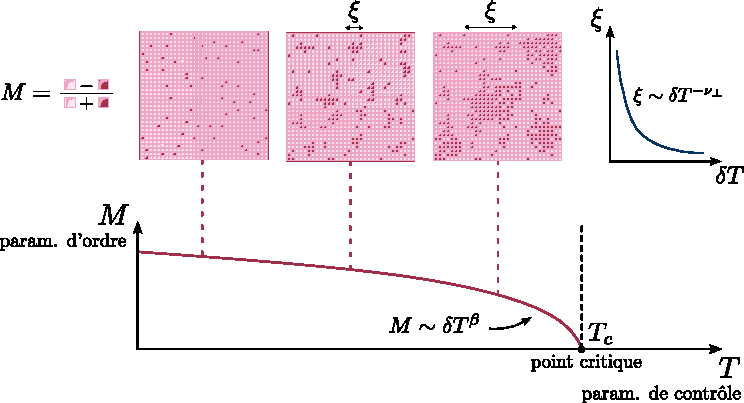
\includegraphics[width=\textwidth]{Chapitre1/Figures/PhenomenesCritiques/PT_conceptCorrLength_fuse.pdf}
	\caption{Illustration de la phénoménologie générale d'une transition de phase via l'exemple de la transition ferromagnétique-paramagnétique.}
	\label{fig:Ising}
\end{figure}

\subparagraph{}Pour conceptualiser le problème, il est d'usage de définir une grandeur, appelée paramètre d'ordre, qui prend des valeurs distinctement différentes dans chacune des phases. La transition se traduit alors par un changement abrupt du paramètre d'ordre autour de la valeur critique du paramètre de contrôle. Dans le cadre de la transition ferromagnétique-paramagnétique, le paramètre d'ordre du système est son aimantation $M$ et le paramètre de contrôle est sa température $T$, dont la valeur critique est la température de Curie $T_c$. Lorsque le matériau est porté à une température $T>T_c$, la phase dominante est la phase paramagnétique, caractérisée par $M=0$, et lorsque celui-ci est refroidi à $T<T_c$ la phase dominante est la phase ferromagnétique, caractérisée par $M\neq 0$ (voir \autoref{fig:Ising}). Le domaine d'étude des phénomènes critiques consiste alors à comprendre l'évolution du système et des quantités le caractérisant près de ce point de transition. Dans la suite de cette sous-section, pour plus de clarté, nous conserverons les notations issues de la transition ferromagnétique-paramagnétique pour développer les concepts associés aux phénomènes critiques.

\subsubsection{Hypothèse de scaling}

\subparagraph{}Afin d'opérer des changements macroscopiques aussi drastiques au cours d'une légère modification du paramètre de contrôle, les entités microscopiques constituant le système doivent coopérer largement proche de la transition. C'est en effet ce que l'on observe : à mesure que l'on s'approche de la transition, la longueur de corrélation $\xi$ associée au système augmente, comme schématisé à la \autoref{fig:Ising}. Au point de transition, aussi appelé point critique, celle-ci diverge.

\subparagraph{}En accord avec ces observations, l'hypothèse de scaling généralisée est une hypothèse fondatrice de l'étude des phénomènes critiques qui permet de comprendre leur phénoménologie \cite{kardar_statistical_2007}. Celle-ci repose sur le fait que, dans le régime critique (i.e. suffisamment proche de la transition), la longueur de corrélation est la seule échelle de longueur pertinente pour décrire le système. En d'autres termes, tous les détails microscopiques du système en-dessous de l'échelle de longueur représentée par $\xi$ sont d'intérêt négligeable. De plus, cette hypothèse suppose que cette longueur de corrélation est une fonction homogène de la distance au point critique :

\begin{equation}
    \xi = \lambda^{\nu_\perp} \tilde{\xi}(\lambda \delta T), \quad \delta T = \frac{T_c-T}{T_c}, \quad \lambda>0.
    \label{eq:homcorr}
\end{equation}

\noindent Le propre d'une fonction homogène étant  que l'\autoref{eq:homcorr} est valide pour tout $\lambda$\footnote{à condition de rester bien sûr dans le domaine critique.}, en prenant $\lambda = 1/\delta T$ nous obtenons :

\begin{equation}
    \xi = \delta T^{-\nu_\perp}\tilde{\xi}(1).
\end{equation}

\noindent Cela retranscrit alors bien le fait que la longueur de corrélation diverge algébriquement avec la distance au point critique.

\begin{figure}[h]
	\centering
	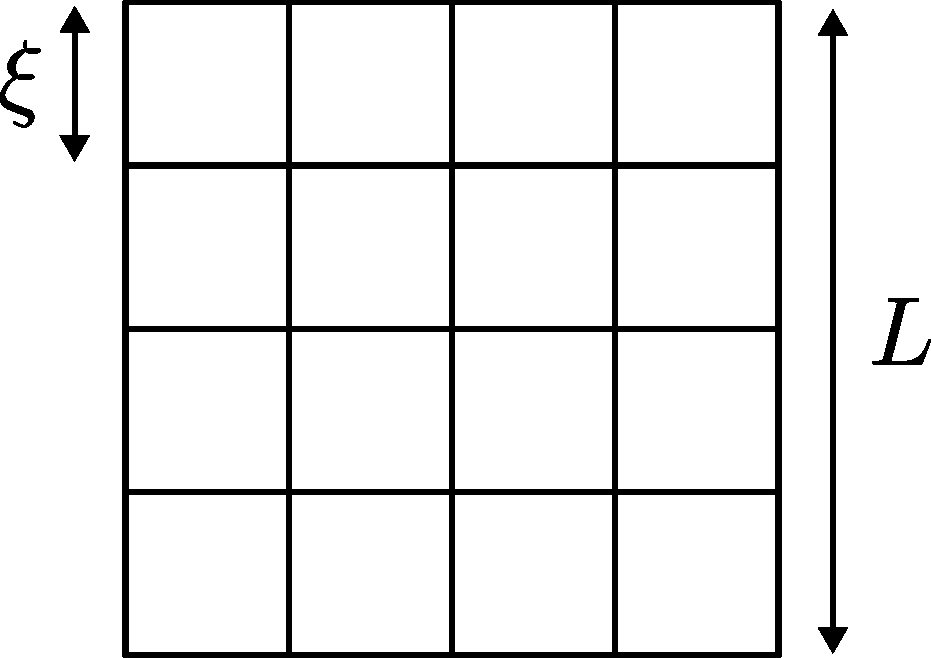
\includegraphics[width=0.3\textwidth]{Chapitre1/Figures/PhenomenesCritiques/decoupageXI.pdf}
	\caption{Découpage schématique d'un système de dimension $L^D$ en une collection de sous-systèmes de dimension $\xi^D$.}
	\label{fig:DecoupageXi}
\end{figure}

\subparagraph{}Cette hypothèse implique un résultat important. Considérons un système de taille $L^D$ que l'on subdivise en un ensemble de sous-compartiments de dimension $\xi^D$, comme représenté à la \autoref{fig:DecoupageXi}. Par définition de la longueur de corrélation, chacun de ces sous-compartiments peut être considéré comme indépendant. Chacun de ceux-ci, au nombre de $\left(\frac{L}{\xi}\right)^D$ contribue à l'énergie libre $f$ du système par la même quantité. En d'autres termes, la partie singulière (associée à la transition) de $f$ se comporte comme $\xi^{-D}$. C'est donc aussi une fonction homogène :

\begin{equation}
    f = \lambda^{y_f}\tilde{f}(\lambda \delta T), \quad \lambda > 0,
\end{equation}

\noindent et dont l'exposant caractéristique est relié au précédent par la relation $y_f = - \nu_\perp D$, génériquement appelée relation d'échelle. 

\subparagraph{}La force de la théorie d'échelle vient alors du point suivant. Les dérivées ou transformées de Legendre d'une fonction homogène sont elles-mêmes des fonctions homogènes. Par ailleurs, celles de l'énergie libre (ou autre potentiel thermodynamique considéré en fonction du système) correspondent à différentes grandeurs physiques d'intérêt. Cela signifie donc que sous cette hypothèse, dans le régime critique, la plupart des quantités décrivant le système sont des fonctions homogènes dont les exposants associés sont liés par des lois d'échelle. Proche du point critique, les observables telles que $\xi$ évoluent donc sans échelle caractéristique, selon des lois de puissance définissant ce qu'on appelle des exposants critiques. Notamment, via le temps de corrélation $\tau$ et la valeur moyenne du paramètre d'ordre $\langle M \rangle$, nous définissons, en plus de $\nu_\perp$, les exposants critiques $\beta$ et $\nu_\parallel$ selon :

\begin{equation}
\begin{aligned}
	\langle M \rangle = \lambda^{-\beta} \tilde{M}(\lambda \delta T) &\Rightarrow \langle M \rangle  \sim \delta T^{\beta},\\
	\tau = \lambda^{\nu_\parallel} \tilde{\tau}(\lambda \delta T) &\Rightarrow \tau \sim \delta T^{-\nu_\parallel}.
\end{aligned}
\end{equation}

\subparagraph{}L'hypothèse de scaling ainsi que les relations d'échelle qui en découlent ont été testées expérimentalement de manière exhaustive, plaçant alors la théorie d'échelle comme le pilier de l'étude des phénomènes critiques \cite{lubeck_universal_2004}.

\subsubsection{Universalité}

\label{sec:univcritique}

\paragraph{Principe}

\subparagraph{}Un aspect essentiel de ce cadre d'étude est de considérer que les détails microscopiques des systèmes situés à des échelles inférieures à $\xi$ ne sont pas pertinents pour en décrire la physique. Dans le régime critique où la longueur de corrélation diverge, ceci motive le fait que le comportement d'une transition peut être déterminé simplement par des considérations globales : c'est le principe d'universalité. L'étude des transitions de phase à l'équilibre a renforcé ce principe d'universalité en montrant que des transitions de nature physique complètement différente partageaient le même comportement critique. Il a alors été possible d'élaborer une catégorisation des phénomènes critiques, les regroupant en classes d'universalité définies uniquement par deux aspects simples (lorsqu'on se limite aux interactions à courte portée) : la dimension de l'espace et les symétries du paramètre d'ordre \cite{kardar_statistical_2007}. Par exemple, la transition ferromagnétique-paramagnétique des matériaux avec un seul axe privilégié d'aimantation appartient à la classe d'universalité d'Ising au même titre que la transition liquide-gaz ou celle de démixtion des liquides binaires \cite{lubeck_universal_2004}. En pratique, cette catégorisation passe par la mesure des exposants critiques, dont chaque ensemble caractérise une unique classe d'universalité.

\paragraph{Théorie continue}

\subparagraph{}Le fait qu'un comportement critique dépende uniquement de critères très généraux motive l'étude de ces phénomènes via des modélisations continues simples sous-forme d'équations de champ.  Par exemple, celle associée à la classe d'Ising est la suivante :

\begin{equation}
	\partial_t \phi (\mathbf{r}, t) = -r\phi (\mathbf{r}, t) + u \phi^3(\mathbf{r}, t) + \kappa\nabla^2 \phi (\mathbf{r}, t) + \sigma\eta(\mathbf{r}, t),
\end{equation}

\noindent avec $\eta$ représentant les fluctuations via un bruit gaussien défini selon :

\begin{equation}
\langle \eta(\mathbf{r}, t) \rangle = 0, \quad \langle \eta(\mathbf{r}, t) \eta(\mathbf{r}^\prime, t^\prime)\rangle = \delta(\mathbf{r}-\mathbf{r}^\prime)\delta(t-t^\prime),
\label{eq:phi4}
\end{equation}

\noindent $\phi$ représentant une version gros grains locale du paramètre d'ordre et $r$ la distance au point critique. Cette théorie continue est connue sous le nom de théorie $\phi^4$ \cite{kardar_statistical_2007}.

\subparagraph{}Dans la limite où les fluctuations de la dynamique sont négligeables, la criticalité décrite par cette équation peut être appréhendée dans son approximation de champ moyen :

\begin{equation}
	\partial_t \phi = -r\phi + u\phi^3 \xrightarrow[r>0]{t\rightarrow \infty} \phi = \left( \frac{r}{u} \right)^\frac{1}{2},
\end{equation}

\noindent menant donc à $\beta^\text{CM} = \frac{1}{2}$. Cependant cette approximation n'est valable que dans certains cas.

\subparagraph{}Dans l'idée que les détails microscopiques ne sont pas pertinents dans le régime critique, nous pouvons redimensionner les distances dans cette équation selon $\mathbf{r}\rightarrow b\mathbf{r}$ avec $b>1$. Sous cette transformation, d'après la théorie d'échelle, les différentes quantités de l'équation sont transformées selon :

\begin{equation}
	\mathbf{r}\rightarrow b\mathbf{r}, \quad t \rightarrow b^{\nu_\parallel/\nu_\perp}t, \quad \phi \rightarrow b^{-\beta/\nu_\perp}\phi,
\end{equation}

\noindent si bien que ce redimensionnement revient à obtenir une équation équivalente à l'\autoref{eq:phi4} avec un redimensionnement des constantes selon :

\begin{equation}
	r \rightarrow b^{\nu_\parallel/\nu_\perp} r, \quad u \rightarrow b^{\nu_\parallel/\nu_\perp - 2\beta/\nu_\perp} u, \quad \kappa \rightarrow b^{\nu_\parallel/\nu_\perp-2}\kappa, \quad \sigma \rightarrow b^{\nu_\parallel/2\nu_\perp+\beta/\nu_\perp - D/2}\sigma.
\end{equation}

\noindent \`A grande échelle ($b\rightarrow\infty$), les fluctuations sont donc négligeables seulement pour $D > (2\beta+\nu_\parallel)/\nu_\perp$. Par ailleurs, dans ce cas champ moyen, l'invariance d'échelle du système au point critique ($r=0$) impose la valeur des exposants $\nu_\parallel^\text{CM} = 1$ et $\nu_\perp^\text{CM} = \frac{1}{2}$. Ce raisonnement définit donc une dimension critique supérieure du système $D_c = 4$ au-delà de laquelle la criticalité décrite par l'équation \autoref{eq:phi4} est triviale\footnote{Nous réutiliserons ce raisonnement générique pour caractériser les propriétés champ moyen d'autres théories dans la suite de cette thèse.}. 

\subparagraph{}En-dessous de cette dimension critique supérieure ($D<D_c$), on ne peut plus négliger les fluctuations dans le système : c'est là que toute la complexité des comportements critiques entre en jeu. Pour étudier le comportement de la théorie de champ à grande échelle dans ce cas, des outils théoriques ont été mis en place. Ceux-ci font intervenir le formalisme associé au groupe de renormalisation. Grâce à ces techniques, il est possible de prédire, au moins perturbativement, les valeurs des exposants critiques associés à une théorie de champ à basse dimension, et donc prédire la criticalité de toute une catégorie de systèmes.

\subparagraph{}En conclusion, les phénomènes critiques à l'équilibre sont caractérisés par des évolutions algébriques des quantités physiques. Ces évolutions sont décrites par différents exposants critiques, reliés par des relations d'échelle. Différentes transitions de phase peuvent être regroupées en une classe d'universalité, décrite par un ensemble de valeurs des exposants critiques. Pour étudier l'universalité de ces classes, il est d'usage de faire appel aux théories de champ continues associées, dont la résolution fait intervenir des outils complexes en-dessous de la dimension critique supérieure.

\subsection{Transitions de phase absorbantes}

\subparagraph{}Après avoir rappelé les bases de la théorie des phénomènes critiques à l'équilibre, nous proposons dans cette sous-section de décrire la phénoménologie propre aux transitions de phase absorbantes. Ces phénomènes hors d'équilibre concernent plus spécifiquement notre étude puisque nous verrons que les transitions de réversibilité et d'écoulement en sont des représentantes. Pour ce faire, nous en proposerons une définition, que nous compléterons ensuite par quelques exemples. Puis, nous présenterons les exposants critiques pertinents pour caractériser ces transitions et la classe d'universalité principale associée.

\subsubsection{Définition}

\subparagraph{}Les transitions de phase absorbantes prennent place dans des systèmes présentant des états absorbants. Ceux-ci correspondent à des états accessibles à la dynamique du système mais dans lesquels celle-ci se retrouve piégée à jamais \cite{lubeck_universal_2004}. Dans une telle transition, le paramètre de contrôle que l'on notera d'abord génériquement $p$ permet de séparer une phase active d'une phase absorbante par sa valeur critique $p_c$. Dans la phase active $p>p_c$, la dynamique du système à temps long est caractérisée par une valeur moyenne positive du paramètre d'ordre $A$, appelé génériquement activité. Dans la phase absorbante $p<p_c$, le système tombe dans un état absorbant au bout d'un temps fini, caractérisé par une activité nulle $A=0$. 

\subparagraph{}La notion d'activité dans ce cadre ne tisse pas de liens avec celle de l'activité dans le contexte de la matière active. Dans une transition de phase absorbante, l'activité correspond plutôt à un état des agents microscopiques qui peut prendre différentes formes selon les systèmes spécifiques considérés.

\subsubsection{Exemples}

\subparagraph{}Sous le point de vue adéquat, de nombreux systèmes peuvent être compris comme des transitions de phase absorbantes. Un exemple incontournable à l'aune de notre époque est celui des épidémies, dans lequel un agent pathogène (virus, bactérie, ...) se propage au sein d'une population \cite{hinrichsen_non_equilibrium_2000, dickman_nonequilibrium_2002, lubeck_universal_2004}. Au premier ordre, on peut modéliser ce système comme à la \autoref{fig:KirbyetArbres}. La population peut alors contenir deux types d'individus : des individus malades, susceptibles de transmettre la maladie à un taux $\lambda$ et de s'en rétablir à un taux $\gamma$, et des individus sains, susceptibles d'être infectés. En fonction de la transmissibilité du virus $\lambda$ et de la capacité de guérison de la population $\gamma$, le système peut connaître deux sorts à temps long : pour $\lambda/\gamma$ suffisamment grand, l'épidémie persistera à temps long alors que pour $\lambda/\gamma$ suffisamment petit, tous les individus finiront par devenir sains. Un tel état est alors un état absorbant puisque dès lors que l'agent pathogène n'a plus de vecteur, il ne peut plus se propager. Dans ce système, on retrouve donc une transition de phase absorbante de paramètre de contrôle $p = \lambda/\gamma$ et dont l'activité correspond à la proportion de personnes infectées dans la population.

\subparagraph{}Un autre exemple pouvant présenter une dynamique tout à fait similaire est celui des feux de forêt \cite{albano_spreading_1995} (voir \autoref{fig:KirbyetArbres}). De la même manière, nous pouvons modéliser ce système au premier ordre par une population d'arbres existant sous deux états possibles : des arbres en feu susceptibles de provoquer l'embrasement d'autres à un taux $\lambda$ et de s'éteindre à un taux $\gamma$, et des arbres sains, seulement susceptibles de prendre feu. Ici encore, selon la valeur du paramètre $p = \lambda/\gamma$, l'état du système à temps long peut prendre deux formes : incendié pour $p>p_c$ et éteint pour $p<p_c$. La forêt sans aucun arbre en feu correspond alors à un état absorbant du système, puisqu'une fois dans cet état, le feu ne peut plus se propager. Dans ce système l'activité correspond à la proportion d'arbres en feu dans la forêt.

\begin{figure}[h]
	\centering
	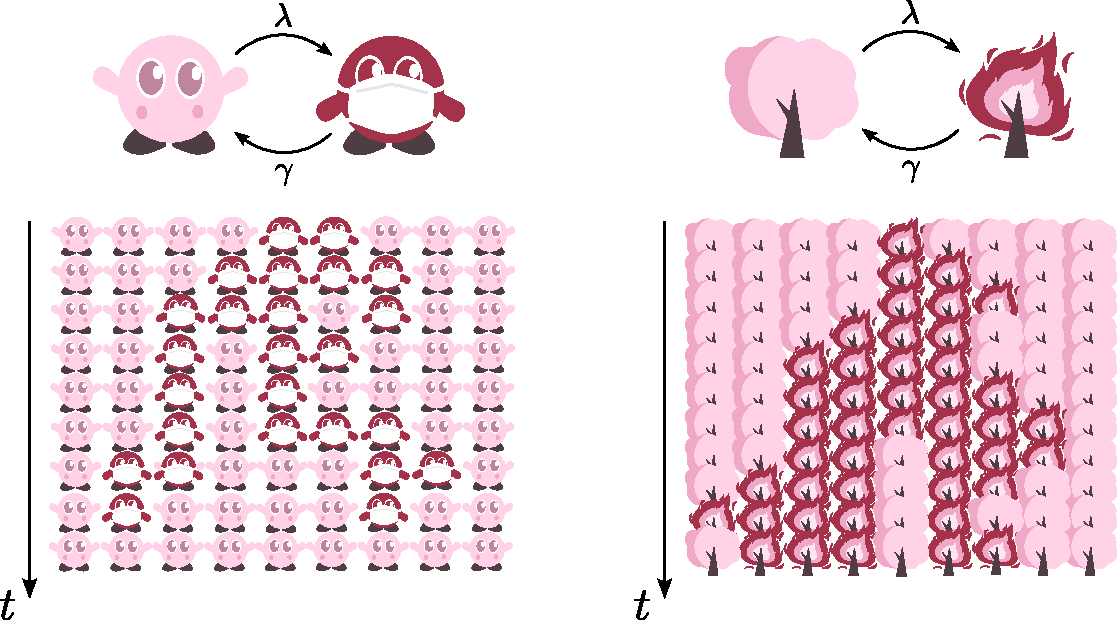
\includegraphics[width=\textwidth]{Chapitre1/Figures/TphiAbs/Kirbies.pdf}
	\caption{Exemples de phénomènes présentant des transitions de phase absorbantes : la propagation des épidémies et les feux de forêts.}
	\label{fig:KirbyetArbres}
\end{figure}

\subparagraph{}De manière générale, de nombreux systèmes peuvent être compris comme des transitions de phase absorbantes s'ils sont observés sous le bon angle. Comme le montrent les exemples précédents, les ingrédients principaux nécessaires à cette dynamique sont une activité microscopique susceptible de se propager comme de s'atténuer et l'existence d'un état bloqué de la dynamique globale.

\subsubsection{Exposants critiques}

\label{sec:tphiexp}

\subparagraph{}Les transitions de phase absorbantes sont des phénomènes hautement hors d'équilibre puisque la présence d'états absorbants implique, par définition, la violation du principe de bilan détaillé. Toutefois, il se trouve que la phénoménologie observée de ces transitions présente de nombreuses similarités avec celle de leurs homologues d'équilibre. Notamment, nous y retrouvons la notion d'homogénéité, d'exposants critiques et d'universalité. Concernant les exposants critiques associés aux transitions de phase absorbantes, ceux-ci peuvent être catégorisés en deux types : ceux reliés à l'état stationnaire de l'activité dans le système, que l'on appellera statiques, et ceux reliés à l'état transitoire ou à des corrélations à deux ou plusieurs temps dans l'état stationnaire, que l'on appellera dynamiques.

\begin{figure}[h]
	\centering
	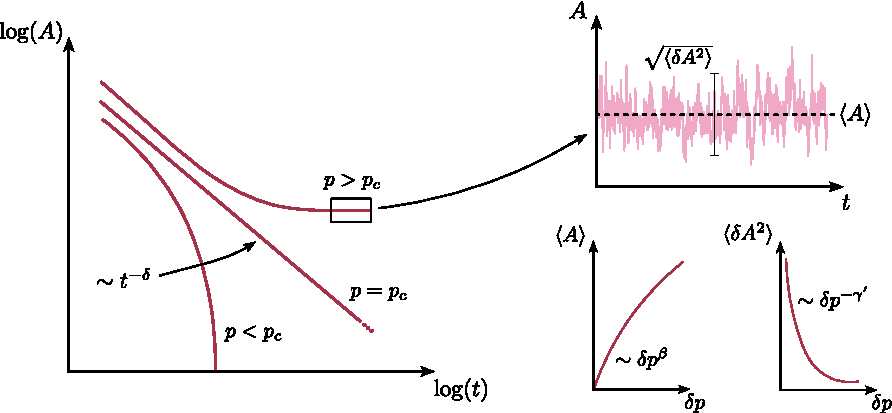
\includegraphics[width=\textwidth]{Chapitre1/Figures/TphiAbs/expabs.pdf}
	\caption{Phénoménologie et définition des différents exposants critiques pertinents dans le cadre des transitions de phase absorbantes.}
	\label{fig:expabs}
\end{figure}

\subparagraph{}Du côté des exposants statiques, nous retrouvons naturellement l'exposant $\beta$ reliant la valeur moyenne de l'activité dans l'état stationnaire à la distance au point critique, et l'exposant $\nu_\perp$ caractérisant la divergence de la longueur de corrélation $\xi$ :

\begin{equation}
	\langle A \rangle \sim \delta p^\beta, \quad \xi \sim \delta p^{-\nu_\perp}, \quad \delta p =  \frac{p-p_c}{p_c}.
\end{equation}

\noindent De plus, nous nous intéresserons aussi dans ce travail à l'évolution des fluctuations du paramètre d'ordre dans l'état stationnaire. Pour un système de taille $L^D$, avec $D$ la dimension du système, nous les caractérisons via la variance $\langle \delta A^2\rangle  = L^D\times(\langle A ^2 \rangle - \langle A \rangle^2)$ dont l'évolution est alors dictée par l'exposant $\gamma^\prime$ :

\begin{equation}
	\langle \delta A^2\rangle \sim \delta p^{-\gamma^\prime}.
\end{equation}

\noindent Le signe apposé à la définition de cet exposant vient du fait qu'en général les fluctuations du paramètre d'ordre divergent à l'approche du point critique, signe d'une dynamique de plus en plus corrélée. En-dessous de la dimension critique $D_c$, les exposants $\beta$, $\gamma^\prime$ et $\nu_\perp$ sont liés par une relation d'échelle :

\begin{equation}
	2\beta + \gamma^\prime = \nu_\perp D,
\end{equation}

\noindent appelée relation d'hyperscaling \cite{lubeck_universal_2004}. Nous ferons appel à cette relation d'échelle à plusieurs reprises dans les différents chapitres de ce manuscrit.

\subparagraph{}Du point de vue dynamique, il existe deux façons principales de caractériser une transition de phase absorbante \cite{lubeck_universal_2004}. La première est de partir d'un état initial avec une zone localisée d'activité, comme c'est le cas sur la \autoref{fig:KirbyetArbres}, et d'étudier la propagation de l'activité dans le système. Une autre possibilité, que nous favoriserons par la suite, est de caractériser la relaxation du système à partir d'un état aléatoire. Dans ce cas, au point critique, la valeur instantanée de l'activité dans le système décroît à temps long de manière algébrique, définissant l'exposant dynamique $\delta$ :

\begin{equation}
	A(t) \sim t^{-\delta}.
\end{equation}

\subparagraph{}Les exposants $\beta$, $\gamma^\prime$ et $\delta$ ainsi définis et illustrés sur la \autoref{fig:expabs} permettent de caractériser une transition de phase absorbante sous différents aspects et de manière unique. 

\subsubsection{Classes d'universalité}

\subparagraph{}Comme à l'équilibre, un grand nombre de transitions de phase absorbantes se regroupent sous forme de classes d'universalité représentées par des valeurs communes des exposants critiques. Dans ce cas hors d'équilibre, la classe d'universalité la plus importante, de manière analogue à la classe d'Ising, est celle de la percolation dirigée (DP) \cite{hinrichsen_non_equilibrium_2000,lubeck_universal_2004}. 

\subparagraph{}Sa dénomination vient de la transition géométrique bien connue qui la représente. Dans le cas de la transition de percolation isotrope, rappelée à la \autoref{fig:percol}-(a), deux sites voisins d'un réseau de $D$ dimensions sont reliés avec une probabilité $p$. Une valeur critique $p_c$ de cette probabilité sépare alors statistiquement deux états du système : pour $p<p_c$ les clusters formés par les liens sont de taille finie tandis que pour $p>p_c$ ceux-ci s'étendent dans tout le système : on dit qu'ils percolent. La percolation dirigée est représentée par le même phénomène, simplement dans ce cas les liaisons entre sites ne peuvent se faire que dans une direction privilégiée (voir \autoref{fig:percol}-(a)). Dans ce cas, les issues possibles en fonction de la valeur du paramètre $p$ sont représentées graphiquement en 2D sur la \autoref{fig:percol}-(b). Nous pouvons alors remarquer de fortes similarités entre la \autoref{fig:percol}-(b) et la \autoref{fig:KirbyetArbres}. En fait, comme lae lecteurice l'aura sûrement déjà compris, les processus absorbants simples présentés précédemment sont équivalents à un phénomène de percolation dirigée, mais dont le temps équivaut à une dimension, soit en $D+1$ dimensions. Une valeur finie de l'activité à temps long dans ces processus correspond alors à la percolation du système tandis que la tombée dans un état absorbant représente la phase non-percolante. Cette équivalence fait que tous ces systèmes sont caractérisés par le même comportement critique : celui de la classe DP.

\begin{figure}[h]
	\centering
	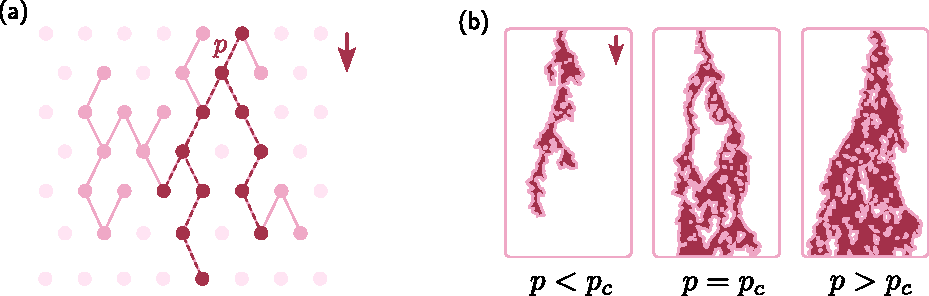
\includegraphics[width=\textwidth]{Chapitre1/Figures/CDP/Percol.pdf}
	\caption{Transition de percolation et de percolation dirigée en 2D. (a) Règles associées à la percolation isotrope (lien roses) et à la percolation dirigée (liens rouges) dont la direction privilégiées est donnée par la flèche. (b) États du système en fonction de la valeur du paramètre de liaison $p$. Pour $p\geq p_c$ le système percole.}
	\label{fig:percol}
\end{figure}

\subparagraph{}Beaucoup d'autres systèmes avec des dynamiques plus complexes ont été caractérisés comme appartenant à la classe DP. Cette ubiquité a motivé une conjecture simple d'appartenance formulée par Janssen et Grassberger \cite{janssen_nonequilibrium_1981, grassberger_phase_1982} : les systèmes présentant une transition de phase absorbante continue vers un unique état absorbant, faisant intervenir des interactions à courte portée et aucune symétrie particulière, appartiennent à la classe DP.

\subparagraph{}D'un point de vue des processus plus abstraits de réaction-diffusion \cite{tauber_applications_2005}, les modèles appartenant à la classe DP peuvent être modélisés par deux processus, un de création et un d’annihilation :

\begin{equation}
A \xrightarrow[]{\lambda} 2A, \quad A \xrightarrow[]{\gamma} \o,
\label{eq:ReacDiffDP}
\end{equation}

\noindent avec $A$ une espèce représentant les agents actifs, diffusant avec un coefficient de diffusion $D_A$. Via cette approche il est possible d'associer, comme pour la classe d'Ising, une théorie de champ à la classe DP :

\begin{equation}
	\partial_t A(\mathbf{r}, t) = rA(\mathbf{r}, t) - uA^2(\mathbf{r}, t) + \kappa\nabla^2 A (\mathbf{r}, t) + \sigma \sqrt{A(\mathbf{r}, t)} \eta(\mathbf{r}, t),
	\label{eq:eqDP}
\end{equation}

\noindent avec la particularité de faire intervenir un bruit multiplicatif (i.e. dépendant de $A$) qui permet de préserver l'existence d'un état absorbant (pour $A=0$, il n'y a plus de fluctuations). Sa forme en $\sim \sqrt{A}$ vient de la stochasticité des réactions, dont la variance est proportionnelle au nombre d'agents microscopiques.  Par une approche d'échelle identique à celle présentée dans le cadre de la théorie de champ de la classe d'Ising, il est possible de déterminer la valeur champ moyen des exposants critiques en-dessous de la dimension critique supérieure $D_c = 4$. Celles-ci sont reportées dans le \autoref{tab:expocrit_DPCDP}. Via des mesures numériques sur des modèles, ou des approches analytiques sur la théorie de champ, la classe DP a aussi été caractérisée précisément en dimension finie. Notamment, nous reportons la valeur des exposants critiques associés en 2D dans le \autoref{tab:expocrit_DPCDP}.

\begin{table}[h]
\centering
\begin{tabular}{ccccc}
\hline \hline Classe & $\beta$ & $\gamma^\prime$ & $\delta$ & $\nu_\perp$ \\
\hline 
\text{DP (en 2D)} & 0.58 & 0.30 & 0.45 & 0.73 \\
\text{CDP (en 2D)} & 0.64 & 0.37 & 0.42 & 0.80 \\
\text{DP/CDP champ moyen} & 1 & 0 & 1 & 0.5 \\
\hline \hline
\end{tabular}
\caption{Valeurs des exposants critiques associés aux classes d'universalité DP et CDP, en 2D et en champ moyen \cite{lubeck_universal_2004}.}
\label{tab:expocrit_DPCDP}
\end{table}

\subparagraph{}Si DP est la classe la plus répandue et la plus caractérisée aussi bien numériquement qu'analytiquement, il existe d'autres classes, cousines de cette première, correspondant à l'ajout d'ingrédients supplémentaires dans les modèles associés. Notamment, celle d'intérêt pour ce travail est celle de la percolation dirigée conservée (CDP), puisqu'elle représente une dynamique très proche de celles mises en place dans la transition de réversibilité et dans la transition vers l'écoulement.

\section{Percolation dirigée conservée}

\subparagraph{}Dans cette section, nous présentons la classe d'universalité CDP de manière exhaustive puisque, comme nous le verrons, elle représente un premier cadre de compréhension des transitions de réversibilité et d'écoulement. De ce fait, cette partie nous permet d'introduire différent concepts comme les dynamiques d'avalanche ou la notion d'hyperuniformité qui nous seront utiles pour caractériser ces transitions d'intérêt. Pour ce faire, nous commencerons tout d'abord par donner les conditions d'appartenance à la classe CDP et les modèles minimaux qu'elle représente. Ensuite, nous introduirons la transition de dépiégeage comme représentante incontournable de cette classe en présentant la riche phénoménologie qui lui est associée. Par correspondance, nous montrerons alors comment la physique de la transition de dépiégeage se retrouve dans les autres modèles théoriques de type CDP. Cela nous permettra de montrer toute la complexité présente dans cette classe d'universalité que l'on retrouvera en partie lors de l'étude des transitions de réversibilité et d'écoulement.

\subsection{Conditions d'appartenance}

\subparagraph{}La classe CDP se démarque de la classe DP par la présence d'un couplage de la dynamique de l'activité à une quantité conservée et d'un nombre infini d'états absorbants. \`A la façon de la conjecture proposée dans le cas de la classe DP, Rossi et al. \cite{rossi_universality_2000} en ont définie une dans le cadre de la classe CDP : tout système stochastique présentant un nombre infini d'états absorbants dans lequel l'activité est couplée à un champ conservé non-diffusif appartient à la classe CDP. \`A cette conjecture s'ajoute implicitement la condition d'interactions uniquement locales, comme formulé dans la conjecture de Grassberger pour la classe DP \cite{grassberger_phase_1982}.

\subparagraph{}Pour comprendre les éléments de cette distinction, il est plus simple de passer directement par la présentation de modèles appartenant à cette classe d'universalité.

\subsection{Modèles représentatifs}

\label{sec:modelesCDP}

\subsubsection{Modèle Manna}

\subparagraph{}Le modèle Manna \cite{manna_two_state_1991} est un modèle emblématique de la classe CDP, si bien qu'il lui en donne parfois le nom (classe d'universalité Manna) \cite{lubeck_universal_2004}. Dans ce modèle, $N$ particules sont disposées sur $L^D$ sites d'un réseau $D$-dimensionnel, chacun de ces sites pouvant accueillir un nombre arbitraire $n$ de particules. De manière générale, ces particules peuvent aussi bien représenter des grains de sable que des paquets d'énergie. La règle dynamique d'un pas de temps à l'autre de l'évolution est alors la suivante : chaque site du réseau accueillant plus de $m$ particules les redistribue aléatoirement aux sites voisins (voir \autoref{fig:Manna}). Ces sites redistribuant la masse qu'ils supportent sont considérés comme actifs.

\begin{figure}[h]
\centering
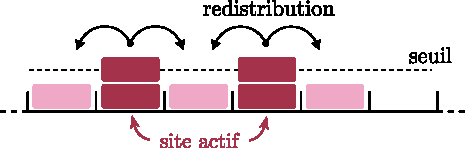
\includegraphics[width=0.6\textwidth]{Chapitre1/Figures/CDP/Manna.pdf}
\caption{Représentation schématique de la dynamique du modèle Manna en 1D. Ici le seuil est fixé à $m=2$.}
\label{fig:Manna}
\end{figure}

\subparagraph{}Sous cette action, les sites sur lesquels a été redistribuée la masse sont susceptibles de dépasser le seuil local $m$ et de devenir actifs à leur tour, menant à une propagation de l'activité dans le système. Ce système présente alors une transition de phase absorbante bien étudiée, dont la densité d'agents $\phi = N/L^D$ est le paramètre de contrôle et dont l'activité $A$ correspond à la proportion de sites actifs du réseau. Pour $\phi > \phi_c$, le système évolue d'un pas de temps à l'autre à travers des configurations avec toujours un excès de particules sur certains sites et donc des redistributions de masse ($A>0$). Cependant, pour $\phi < \phi_c$, le système finit par tomber à temps long dans un état où tous les sites sont inactifs et donc d'activité nulle $A=0$. Un tel état est un état absorbant puisque dès lors qu'aucune redistribution n'a lieu, aucun site ne peut devenir actif. 

\subparagraph{}Dans les modèles épidémiques et de feux de forêts présentés précédemment, il existe un unique état absorbant (toute la population est guérie ou toute la forêt est éteinte). Dans le modèle Manna, il en existe plusieurs. En effet, tout état où tous les sites vérifient $n<m$ sont des états absorbants de la dynamique. Dans la limite thermodynamique $L\rightarrow \infty$, il y en a une infinité. Cela remplit donc la première condition de la conjecture de Rossi et al. \cite{rossi_universality_2000}. Par ailleurs, la dynamique d'activité des sites du réseau est couplée à la dynamique des $N$ particules, dont le nombre est conservé à chaque instant. Dans une vision à grande échelle, ces $N$ particules constituent un champ de densité $\rho (\mathbf{r}, t)$ de valeur intégrale constante (donc dit conservé) et évoluant uniquement sous l'action de l'activité (donc dit non-diffusif). Cela remplit donc la seconde condition de la conjecture, faisant du modèle Manna un représentant de la classe CDP. Chronologiquement cependant, c'est en réalité plutôt le modèle Manna qui a permis de définir la classe CDP \cite{lubeck_universal_2004}.

\subsubsection{Random Organization Model}

\subparagraph{}Un second modèle respectant la conjecture de Rossi et al. \cite{rossi_universality_2000} et appartenant à la classe CDP est le Random Organization Model (ROM) \cite{corte_random_2008, tjhung_criticality_2016}. Le ROM est très proche du modèle Manna dans son principe et sa dynamique, à la différence que celle-ci a lieu dans un espace continu.

\begin{figure}[h]
\centering
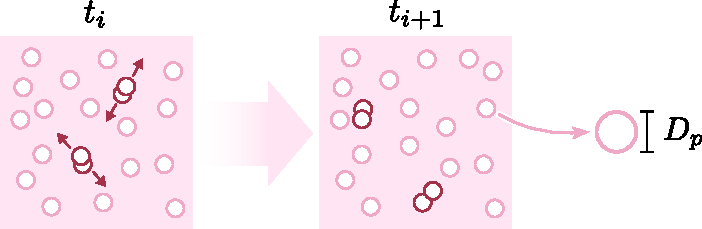
\includegraphics[width=0.85\textwidth]{Chapitre1/Figures/CDP/ROM.pdf}
\caption{Représentation schématique de la dynamique du ROM en 2D.}
\label{fig:ROM}
\end{figure}

\subparagraph{}Dans le cadre de ce modèle, $N$ particules sphériques de diamètre $D_p$ sont positionnées dans un espace de $D$ dimensions et d'extension spatiale $L$. Chacune de ces $N$ particules peut alors prendre deux états à chaque pas de temps : si la particule se recouvre avec une autre particule elle est active, sinon elle est passive. Lorsqu'une particule est active, celle-ci est soumise à un déplacement d'amplitude aléatoire, modifiant sa position dans l'espace continu. Ce déplacement représente alors la possibilité d'un recouvrement avec une nouvelle particule, menant à une potentielle propagation de l'activité dans le système. Cette dynamique présente une transition de phase absorbante dont le paramètre d'ordre est la fraction volumique $\phi$ de particules dans le système et dont l'activité $A$ correspond à la proportion de particules actives. Pour $\phi>\phi_c$, le système traverse des configurations où il existe toujours au moins un recouvrement entre particules ($A>0$). Cependant, pour $\phi<\phi_c$, le système finit par tomber dans une configuration où toutes les particules sont suffisamment éloignées pour qu'aucunes ne se recouvrent ($A=0$). Une telle configuration est un état absorbant puisque sans le déplacement d'une particule active, aucune particule passive ne peut le devenir. 

\subparagraph{}Comme dans le cas du modèle Manna, le ROM possède un nombre infini d'états absorbants. En effet, chaque ensemble de position des particules $\{\mathbf{r}_i\}_{i<N}$ vérifiant $|\mathbf{r}_i-\mathbf{r}_j|<D_p$ pour tout $i\neq j$ est un état absorbant. Les positions étant continues, il y en a une infinité (et pas seulement dans la limite thermodynamique). Le ROM vérifie donc la première condition de la conjecture de Rossi et al. \cite{rossi_universality_2000}. Par ailleurs, de la même manière que dans le modèle Manna, ce modèle fait intervenir la dynamique non-diffusive de $N$ particules dont le nombre est conservé à chaque instant, vérifiant de ce fait la seconde condition de la conjecture. La seule différence ici est que l'activité est aussi représentée par les particules (actives) et non l'espace (comme c'est le cas dans le modèle Manna via la notion de sites actifs). Ce modèle est donc aussi un représentant de la classe CDP.

\subparagraph{}Par définition d'une classe d'universalité le modèle Manna et le ROM sont donc caractérisés par la même théorie sous-jacente, associée à un ensemble cohérent d'exposants critiques.

\subsection{Comportement critique}

\label{sec:CompCDP}

\subparagraph{}Du point de vue des processus de réaction-diffusion, les modèles appartenant à la classe CDP peuvent être ramenés à un processus à deux espèces \cite{van_wijland_wilson_1998, pastor_satorras_reaction_diffusion_2001, pastor_satorras_field_2000} (contrairement à la classe DP qui n'en fait intervenir qu'une) :

\begin{equation}
	A +B \xrightarrow[]{\lambda} 2A, \quad A \xrightarrow[]{\gamma} B,
\end{equation}

\noindent avec l'espèce $A$ diffusant avec un coefficient de diffusion $D_A$. Ces deux processus conservent alors le nombre total $N=N_A+N_B$ de particules, comme c'est le cas dans le modèle Manna et le ROM. Via ce formalisme, il est possible de définir une théorie de champ décrivant cette dynamique proche de celle de DP \cite{van_wijland_universality_2002, le_doussal_exact_2015} :

\begin{equation}
\begin{aligned}
	&\partial_t A(\mathbf{r}, t) = (\omega\rho (\mathbf{r}, t) - r)A(\mathbf{r}, t) - uA^2(\mathbf{r}, t) + \kappa\nabla^2 A (\mathbf{r}, t) + \sigma \sqrt{A(\mathbf{r}, t)} \eta(\mathbf{r}, t),\\
	&\partial_t \rho (\mathbf{r}, t) = \kappa\nabla^2 A (\mathbf{r}, t),
\end{aligned}
\label{eq:CDP}
\end{equation}

\noindent avec $\rho(\mathbf{r}, t)$ le champ conservé.

\subparagraph{}Via une analyse d'échelle similaire au cas DP, il est possible de montrer que la classe CDP admet des exposants de champ moyen identiques en-dessous de la même dimension critique supérieure $D_c = 4$ \cite{le_doussal_exact_2015, lubeck_universal_2004}. Ainsi, en champ moyen, les classes DP et CDP sont équivalentes. Pour $D<D_c$ cependant, les mesures numériques sur les différents modèles représentant la classe CDP ont permis de la séparer de son homologue DP. En 2D, les valeurs des exposants déterminés pour cette classe sont reportées dans le \autoref{tab:expocrit_DPCDP}.

\subparagraph{}Comme on peut le remarquer, les exposants critiques caractérisant les deux transitions sont en fait très similaires, avec un écart relatif de seulement quelques pourcents. Cette grande proximité a rendu compliquée la séparation de ces deux classes, qui a alors été un sujet de débats. Toutefois, les techniques numériques actuelles et des arguments analytiques basés sur les techniques du groupe de renormalisation permettent aujourd'hui d'affirmer que ces deux criticalités sont bien distinctes.

\subsection{Classe CDP et transition de dépiégeage}

\subparagraph{}En dehors des modèles de particules comme le modèle Manna ou le ROM, la classe CDP possède une forte représentation, notamment en matière molle, via la transition de dépiégeage. Dans cette sous-section, nous proposons de présenter succinctement la transition de dépiégeage. Pour ce faire, nous en donnerons d'abord une image générale dans le cadre théorique des variétés élastiques. Cela nous permettra d'en décrire la phénoménologie associée, notamment via la rugosité de l'interface et la dynamique d'avalanche. Nous ferons ensuite le parallèle entre transition de dépiégeage et la classe CDP en expliquant l'équivalence récemment mise en évidence entre ces deux objets.

\subsubsection{Phénoménologie de la transition de dépiégeage}

\paragraph{Une transition de phase absorbante}

\subparagraph{}Dans un cadre général, la transition de dépiégeage concerne le mouvement d'une variété élastique de $D$ dimensions dans un milieu désordonné de $D+n$ dimensions \cite{fisher_collective_1998}. Au cours de celui-ci, deux phénomènes entrent en jeu. D'une part, l'élasticité de la variété tend à rapprocher localement chacun de ses points. D'autre part, le milieu désordonné agit sur chaque point de la variété en le piégeant  localement, plus ou moins fortement. L'exemple le plus parlant est celui-ci d'une ligne élastique ($D=1$) se déplaçant sur une interface rugueuse ($n=1$), comme représenté à la \autoref{fig:depinningbase}-(a).

\begin{figure}[h]
	\centering
	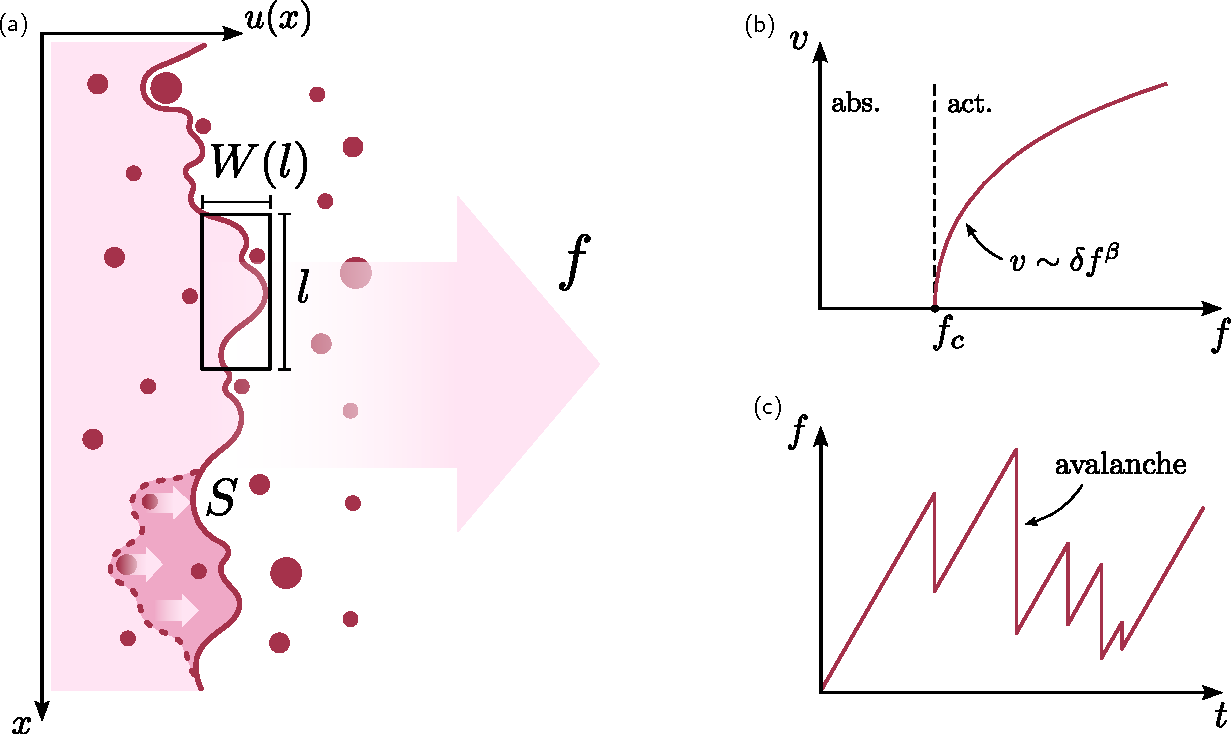
\includegraphics[width=\textwidth]{Chapitre1/Figures/Depinning/depinningbase.pdf}
	\caption{(a) Représentation schématique de la dynamique à l’œuvre dans la transition de dépiégeage en 1D, i.e. dans le cas d'une ligne élastique. Les disques rouges représentent le substrat désordonné. (b) Évolution de la vitesse moyenne de l'interface en fonction de la force appliquée (c) Dynamique d'avalanche dans le cadre d'un processus de forçage-dissipation. Chaque chute de force globale représente une avalanche dans la ligne élastique.}
	\label{fig:depinningbase}
\end{figure} 

\subparagraph{}Sous l'action d'une force extérieure $f$, matérialisée par une densité de force uniforme le long de la ligne,  celle-ci peut se dépiéger localement de l'interaction avec le substrat et se déplacer jusqu'au prochain point de piégeage. Ce déplacement induit une nouvelle configuration de la ligne et modifie alors la force élastique à laquelle sont soumis les autres points. Si l'addition de cette nouvelle force élastique locale et de la force extérieure est suffisamment grande, un autre point de la ligne peut se dépiéger et avancer. Cela constitue un mécanisme de propagation du dépiégeage. Il y a alors deux cas possibles en regard du comportement global de la ligne. Pour une force extérieure suffisamment grande $f>f_c$, le système se dépiège localement en permanence, amenant dans l'état stationnaire à une vitesse moyenne de déplacement de l'interface non-nulle $v>0$. Cependant, pour une force extérieure trop faible $f<f_c$, le système finit par tomber dans un état totalement piégé : localement l'addition de la force extérieure et de la force élastique ne permet pas de contrer la force de piégeage exercée par le substrat. 

\subparagraph{}Cette transition, entre un état mobile et un état piégé, est ce qu'on appelle la transition de dépiégeage. Comme lae lecteurice l'aura sûrement déjà compris, cette transition peut être abordée comme une transition de phase absorbante dont le paramètre de contrôle est la force extérieure $f$ et dont l'activité correspond à la vitesse de l'interface $v$ (localement, un point de l'interface est actif s'il se déplace). 

%L'état piégé correspond effectivement à un état absorbant puisque, en l'absence de fluctuations thermiques que l'on ne considérera pas dans ce travail, il est impossible qu'un point de la ligne se dépiège sans ajout supplémentaire de force.

\subparagraph{}Dans la suite de cette partie, nous présentons deux caractéristiques incontournables de la criticalité associée à la transition de dépiégeage : la rugosité de l'interface et la dynamique d'avalanche.

\paragraph{Rugosité}

\subparagraph{}La compétition complexe entre force de rappel élastique qui tend à aplanir l'interface et force de piégeage qui tend à déformer l'interface rend la structure de cette dernière non-triviale : proche de la transition, elle acquiert une certaine rugosité \cite{fisher_collective_1998, wiese_theory_2022}. La rugosité d'une interface est définie via la largeur $W$ balayée par une portion d'extension $l$ de cette interface (voir \autoref{fig:depinningbase}-(a)). Proche de la transition, $W$ varie algébriquement avec $l$ selon :

\begin{equation}
	W(l) \sim l^\eta,
\end{equation}

\noindent $\eta$ définissant l'exposant de rugosité, un exposant universel au même titre qu'un autre exposant critique. En définissant $u(x)$ la position de l'interface, cette évolution algébrique se retrouve de manière équivalente dans les fluctuations de cette position. En effet, on a directement :

\begin{equation}
	W^2(l) = \overline{\left\langle (u(\mathbf{r}) - \langle u(\mathbf{r}) \rangle)^2\right\rangle} \sim l^{2\eta},
\end{equation}

\noindent où $\langle \cdot \rangle$ désigne la moyenne spatiale sur la portion d'extension $l$ et $\overline{\cdot}$ la moyenne sur les réalisations du désordre. Dans l'espace de Fourier\footnote{Les notations et conventions utilisées dans ce manuscrit pour la transformée de Fourier sont indiquées dans l'\annexeref{sec:conv_fourier}.}, cette propriété se retrouve dans le facteur de structure $S$ : 

\begin{equation}
	S(\mathbf{q}) = \overline{\hat{u}(\mathbf{q})\hat{u}(-\mathbf{q})} \sim q^{-(D+2\eta)}.
\end{equation}

\paragraph{Avalanches}

\subparagraph{}En partant d'une configuration piégée de la ligne élastique et en augmentant lentement la force extérieure $f$ tout en gardant $f<f_c$, la ligne finit par se dépiéger localement, et une portion de celle-ci se déplace avant de se retrouver bloquée à nouveau. Ce saut d'un état absorbant à un autre est ce qu'on appelle une avalanche. Ces objets sont définis par leur taille $S$, correspondant au déplacement moyen de la ligne lors de l'évènement, et leur durée $T$. Proche du point critique $f=f_c$, ces caractéristiques sont distribuées algébriquement selon \cite{narayan_threshold_1993, rosso_avalanche_size_2009, le_doussal_statistics_2009, le_doussal_size_2009, wiese_theory_2022} :

\begin{equation}
P_S(S) \sim S^{-\tau}g_S\left( \frac{S}{S_c} \right), \quad P_T(T) \sim T^{-\tau^\prime}g_T\left( \frac{T}{T_c} \right),
\end{equation}

\noindent avec $g_S(x)$ et $g_T(x)$ constantes pour $x\ll 1$ et à décroissance rapide pour $x>1$, $\tau$ et $\tau^\prime$ définissant des exposants d'avalanche universels. Ces deux quantités peuvent être reliées à l'extension spatiale $l$ de l'avalanche par deux nouveaux exposants critiques :

\begin{equation}
	S \sim l^{d_f}, \quad T \sim l^z,
\end{equation}

\noindent avec $d_f$ la dimension fractale des avalanches et $z$ l'exposant dynamique. Ces deux exposants sont reliés à deux autres exposants présentés précédemment par les relations d'échelle :

\begin{equation}
	d_f = D + \eta, \quad z = \frac{\nu_\parallel}{\nu_\perp}.
\end{equation}

\subparagraph{}Pour $f>f_c$, la dynamique se prolonge indéfiniment et il est donc complexe de séparer les différentes avalanches. Pour analyser les avalanches au-dessus de la force critique il est alors d'usage de procéder d'une manière un peu différente : en plus du mécanisme de forçage, un mécanisme de dissipation est ajouté. Cette fois, en parallèle d'une augmentation constante de $f$, la force extérieure suit une diminution instantanément proportionnelle à l'activité globale dans le système \cite{le_priol_long_range_2020, wiese_theory_2022}. Lorsque l'augmentation de $f$ est suffisamment lente, une séparation d'échelle se crée entre le forçage et la relaxation du système d'un état piégé à un autre. Les évènements de relaxation ainsi désignés sont associés aux avalanches au-dessus du seuil (voir \autoref{fig:depinningbase}-(c)). De la même façon, il est possible d'en caractériser la statistique via la taille et la durée des évènements. Sous ces conditions, le système évolue naturellement vers le point critique $f=f_c$. On parle alors de criticalité auto-organisée (SOC) \cite{bak_self_organized_1988, turcotte_self_organized_1999, lubeck_universal_2004}. Dans ce cadre, les cut-offs des distributions ne dépendent que de l'extension spatiale $L$ du système selon :

\begin{equation}
	S_c \sim L^{d_f}, \quad T_c \sim L^{z}.
\end{equation}

\subsubsection{Mapping avec la classe CDP}

\label{sec:mapping_dep_cdp}

\subparagraph{}L'intérêt de présenter la transition de dépiégeage dans le cadre de notre travail est que toute la richesse de ce phénomène longuement étudié se retrouve dans les modèles appartenant à la classe CDP. En effet, nous présentons dans cette partie les travaux de Le Doussal et Wiese qui montrent que la transition de dépiégeage peut être directement mise en équivalence avec l'universalité de la percolation dirigée conservée \cite{le_doussal_exact_2015, wiese_hyperuniformity_2024}.

\subparagraph{}La transition de dépiégeage peut être modélisée simplement par une équation du mouvement continue sur la ligne. Dans le cas où l'élasticité de la ligne est à courte portée, celle-ci prend la forme suivante \cite{fisher_collective_1998, wiese_theory_2022} :

\begin{equation}
	\partial_t u (x,t) = (\nabla^2 - m^2)u(x,t) + F(x, u(x,t)) + f(x,t), \quad F(x,u) = - \partial_u V(x,u),
	\label{eq:qEW}
\end{equation}

\noindent avec $u$ la position de l'interface perpendiculairement à l'axe $(Ox)$, $f$ la force extérieure et $F$ la force aléatoire de piégeage, dérivant d'un potentiel désordonné $V$. Dans la limite $m=0$, celle-ci correspond à l'équation de quenched-Edward-Wilkinson \cite{nattermann_dynamics_1992}. Le terme $\nabla^2 u (x,t)$ représente la force élastique de courte portée le long de la ligne. De manière générale, nous pouvons écrire ce terme via la formulation $(\mathcal{G}\ast u) (x,t)$ désignant la convolution du champ de déplacement avec un propagateur de redistribution élastique $\mathcal{G}$. Ceci peut s'avérer utile dans le cas de la généralisation aux interactions à longue portée, discutées dans la suite de cet ouvrage.

\subparagraph{}Par cette formulation, il a été possible de faire une équivalence entre l'\autoref{eq:qEW} et l'\autoref{eq:CDP}, associant alors directement la transition de dépiégeage à la classe d'universalité CDP \cite{le_doussal_exact_2015, wiese_hyperuniformity_2024}. Dans ce cadre, le champ d'activité $A$ correspond naturellement au champ de vitesse de l'interface $\partial_t u$. La correspondance moins évidente que montre cette équivalence est celle entre la densité de particules $\rho(x,t)$ dans la théorie CDP et la force de rappel élastique dans le cadre théorique du dépiégeage :

\begin{equation}
	\rho(x,t) - \rho_0 \sim \nabla^2 u (x,t),
	\label{eq:equivCDPdépiégeage}
\end{equation}

\noindent où $\rho_0$ représente la densité moyenne de particules. Cette correspondance permet de faire un lien entre les deux mécanismes de propagation de l'activité. Dans un modèle de particules comme le modèle Manna, l'activité induit localement une redistribution de la masse (représentée par $\rho(x,t)$), susceptible de générer de l'activité par surcharge de nouveaux sites. De manière équivalente, dans le cas du dépiégeage, l'activité induit localement une redistribution de la force élastique susceptible de générer de l'activité par traction suffisante de nouveaux points de la ligne.

\subparagraph{}L'étude de la transition de dépiégeage via sa théorie continue a été réalisée de manière extensive, numériquement mais aussi analytiquement via la mise en place d'outils du groupe de renormalisation fonctionnel. Cette équivalence permet alors de transposer tous les résultats obtenus à la théorie CDP, comme la valeur des exposants critiques associés. De plus, ce mapping permet de faire le lien entre les différentes propriétés de la transition de dépiégeage et celles des modèles de particules, notamment celles de rugosité et de dynamique d'avalanche. Dans la suite de cette section, nous proposons d'expliciter l'équivalent de ces propriétés dans les modèles de particules puisque ces notions nous seront utiles dans la suite de cette ouvrage.

\subsection{Avalanches}

\label{sec:IntroAvalanches}

\subparagraph{}De la même manière que dans la transition de dépiégeage, il est possible d'observer des avalanches dans les modèles de particules appartenant à la classe CDP \cite{lubeck_moment_2000, dickman_paths_2000}. La façon la plus courante de les étudier est, comme dans le cas du dépiégeage, d'ajouter au modèle une composante de forçage et de dissipation \cite{lubeck_universal_2004}. Prenons l'exemple du modèle Manna. Dans ce cas, le forçage correspond à l'augmentation progressive de la densité de particules, via l'ajout aléatoire à un taux $\kappa$ de particules dans le système. La dissipation correspond, elle, à une disparition des particules sur les sites actifs à un taux $\tau$. Dans la limite $\kappa/\tau \ll 1$, la séparation d'échelle entre le forçage et la dissipation fait place à un phénomène d'avalanche : le système saute d'un état inactif à un autre, via des impulsions d'activité. Via ce processus, le système oscille naturellement autour de sa densité critique $\phi_c$.

\subparagraph{}De la même manière que dans la transition de dépiégeage, ces avalanches peuvent être caractérisées via leur taille et leur durée et les exposants critiques $\tau$, $\tau^\prime$, $d_f$ et $z$ qu'elles définissent. Ces deux transitions étant équivalentes, elles partagent les mêmes valeurs de ces exposants. Dans le cas des modèles de particules, la taille d'une avalanche correspond à la quantité d'activations générées lors de la relaxation $S = \int_0^T \mathrm{d}t~ A(t)$.

\subparagraph{}Dans le cadre de la classe CDP, il est possible de relier les exposants d'avalanches aux exposants critiques dynamiques \cite{munoz_avalanche_1999, lubeck_universal_2004}, reliant sans équivoque la dynamique critique à densité imposée à celle sous le mécanisme de forçage-dissipation. Ainsi, l'étude des avalanches revient à étudier la dynamique de la transition d'un point de vue différent de celui présenté à la \autoref{sec:tphiexp}.

\subsection{Hyperuniformité}

\label{sec:introHU}

\paragraph{Fluctuations de position, fluctuations de densité}

\subparagraph{}La rugosité est une propriété propre aux interfaces. Il n'est donc pas direct de voir comment son aspect critique se transpose aux modèles de particules. En fait, l'équivalence soulignée dans l'\autoref{eq:equivCDPdépiégeage} reliant la densité de particules $\rho$ à la position de l'interface $u$ permet de faire le lien entre fluctuations de position et fluctuations de densité :

\begin{equation}
	\overline{\left\langle (\rho(\mathbf{r}) - \langle \rho(\mathbf{r}) \rangle)^2\right\rangle} \rightarrow \overline{\left\langle (\nabla^2 u(\mathbf{r}) - \langle \nabla^2 u(\mathbf{r}) \rangle)^2\right\rangle} \sim l^{2(\eta-2)},
	\label{eq:MappingHyperuni}
\end{equation}

\noindent avec $l$ l'extension spatiale du domaine considéré pour la mesure des fluctuations. Un exposant de rugosité $\eta$ non-trivial implique donc des fluctuations de densité non-triviales dans les modèles de particules appartenant à la classe CDP. Dans une certaine limite, cette propriété correspond à une hyperuniformité de la répartition de masse dans le système. Pour le comprendre, nous introduisons brièvement ce qu'est l'hyperuniformité dans un cadre général.

\paragraph{Répartition de masse et hyperuniformité}

\subparagraph{}La répartition d'un ensemble de points dans l'espace peut prendre différentes formes, associées à différents types de corrélations. Celle-ci peut aller de la structure cristalline infiniment corrélée au cas aléatoire totalement décorrélé. Une manière de quantifier le degré de corrélation spatiale est d'étudier comment évoluent les fluctuations de densité à différentes échelles du système. 

\subparagraph{}Dans le cas d'une répartition poissonienne totalement décorrélée (voir \autoref{fig:HU}-(b)), la variance $\langle \delta n^2 \rangle$ du nombre $n$ de particules dans un échantillon évolue proportionnellement à son extension spatiale $l^D$. Considérant des répartitions uniformes, on a par ailleurs $\langle n \rangle \sim l^D$. Ainsi dans ce cas décorrélé on a :

\begin{equation}
	\langle \delta n^2 \rangle_l \sim \langle n \rangle_l.
\end{equation} 

\subparagraph{}Dans le cas d'un ordre parfaitement cristallin (voir \autoref{fig:HU}-(a)), la variance $\langle \delta n^2 \rangle$ évolue proportionnellement au périmètre de la zone considérée\footnote{Ceci est valable tant que la forme du domaine n'est pas spécifiquement reliée au motif cristallin.}, lui même évoluant comme $l^{D-1}$. Ainsi, on aura :

\begin{equation}
	\langle \delta n^2 \rangle_l \sim \langle n \rangle_l^{1-1/D}.
\end{equation} 

\subparagraph{}Une évolution non-linéaire de $\langle \delta n^2 \rangle$ avec $\langle n \rangle$ indique la présence de corrélations dans la répartition de la densité dans le système. Si le cas cristallin est le plus extrême, il existe un continuum de répartitions caractérisées par $\langle \delta n^2 \rangle_l \sim \langle n \rangle_l^{\sigma}$, indiquant la présence de corrélations intermédiaires. Dès lors que $\langle \delta n^2 \rangle$ croît moins rapidement que $\langle n \rangle$ avec $l$ (i.e. $\sigma < 1$), on qualifie cette répartition d'hyperuniforme.

\begin{figure}[h]
	\centering
	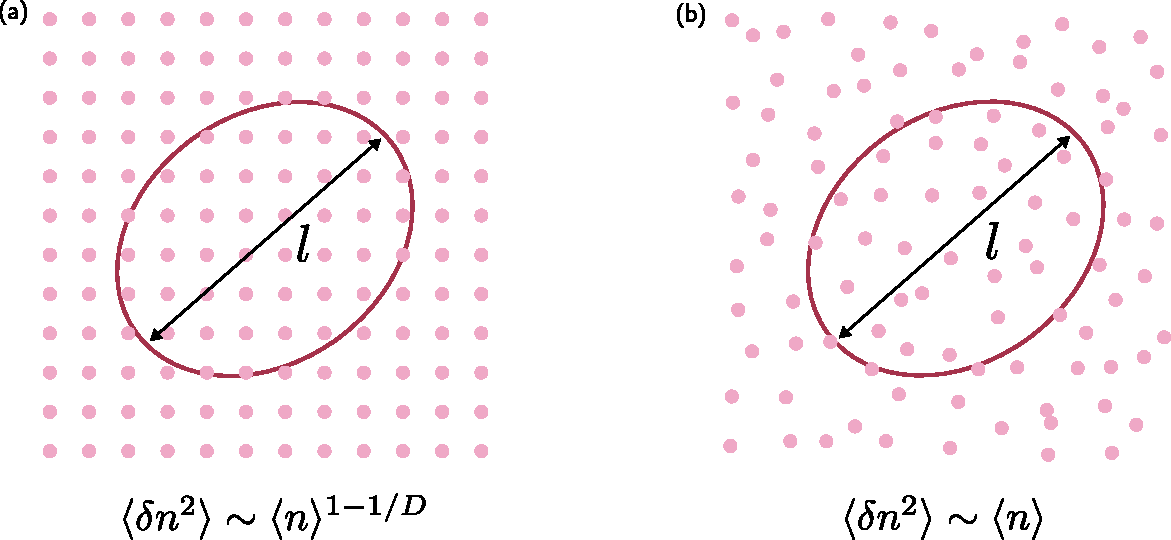
\includegraphics[width=\textwidth]{Chapitre1/Figures/CDP/hyperuniformite.pdf}
	\caption{Répartitions de masse dans le cas cristallin (a) et dans le cas poissonien (b), amenant à des lois d'échelle différentes entre $\langle \delta n^2 \rangle$ et $\langle n \rangle$.}
	\label{fig:HU}
\end{figure}

\paragraph{Hyperuniformité dans les modèles de particules appartenant à la classe CDP}

\subparagraph{}Dans un modèle de particules, il est possible d'associer trivialement les fluctuations de nombre de points/particules aux fluctuations de densité. Ainsi, via l'\autoref{eq:MappingHyperuni}, les exposants $\sigma$ et $\eta$ sont en fait directement liés par la relation d'échelle :

\begin{equation}
	\sigma = 2 + \frac{2\eta - 4}{D}.
	\label{eq:rel_eta_sigma}
\end{equation}

\noindent Un exposant de rugosité $\eta < 1$ dans le modèle de dépiégeage correspond donc de manière équivalente à une répartition hyperuniforme de la masse dans les modèles de particules en 2D. En dimension arbitraire, une évolution hyperuniforme $\sigma < 1$ est associée à un exposant de rugosité $\eta < (4-D)/2$. Cette équivalence est validée par les mesures effectuées sur les modèles numériques. Par exemple, dans le cas du ROM en 2D, il a été mesuré $\sigma \approx 0.775$ \cite{tjhung_hyperuniform_2015, hexner_hyperuniformity_2015, weijs_emergent_2015}.

\subsection{Bilan}

\subparagraph{}En conclusion, la classe d'universalité CDP prétend à représenter tous les modèles présentant une transition de phase absorbante avec une infinité d'états absorbants et impliquant la dynamique d'un champ conservé. Cette classe possède deux représentations principales : les modèles de particules comme le modèle Manna ou le ROM et les modèles de dépiégeage. Les phénomènes apparentés à cette classe présentent une phénoménologie riche, caractérisée par des propriétés hyperuniformes et une dynamique d'avalanche critique. Via l'étude combinée des modèles de particules et de la transition de dépiégeage, le cadre CDP représente un objet d'étude bien balisé, regroupant prédictions théoriques et mesures numériques dans différentes dimensions. L'intérêt d'avoir présenté cette classe exhaustivement est qu'elle correspond en fait à un cadre de description proche des transitions qui motivent ce travail : la transition de réversibilité dans les suspensions cisaillées cycliquement et la transition vers l'écoulement des fluides à seuil. Les aspects spécifiques de la dynamique associée (avalanches, hyperuniformité, ...) se retrouveront donc dans notre étude de ces phénomènes.

\section[Les transitions de réversibilité et d'écoulement comme transitions de phase \\ absorbantes]{Les transitions de réversibilité et d'écoulement comme transitions de phase absorbantes}

\subparagraph{}Dans cette section, nous revenons sur les deux objets d'intérêt de notre travail : la transition de réversibilité dans les suspensions cisaillées cycliquement et la transition vers l'écoulement des fluides à seuil. Pour chacune d'elle, nous explicitons la dynamique sous-jacente à ces transitions et expliquons en quoi celle-ci correspond à celle d'une transition de phase absorbante. Puis, en se basant sur la conjecture de Rossi et al. \cite{rossi_universality_2000}, nous montrons que ces deux systèmes sont proches de ceux représentés par la classe CDP, seulement avec la présence additionnelle d'interactions à longue portée.

\subsection{Transition de réversibilité}

\subparagraph{}Dans la première partie de l'introduction, nous avions présenté la transition de réversibilité dans les suspensions cisaillées cycliquement comme séparant un état réversible, stroboscopiquement arrêté, d'un état irréversible, stroboscopiquement diffusif. Pour comprendre comment ce phénomène peut être appréhendé dans le cadre des transitions de phase absorbantes, il est nécessaire de remarquer comment cette diffusion stroboscopique prend place.

\subsubsection{La diffusion comme une succession d'interactions irréversibles}


\subparagraph{}Dans la limite de bas Reynolds, les équations de Stokes qui gouvernent la dynamique de ce système sont réversibles dans le temps \cite{kimMicrohydrodynamicsPrinciplesSelected1991}. En d'autres termes, si lors de la première moitié d'un cycle une particule n'est déplacée que par les mouvements réversibles du fluide, alors lors de la seconde moitié de ce cycle, elle reviendra à sa position initiale. Toutefois, si au cours de cette première moitié de cycle la particule interagit irréversiblement avec une autre particule à courte portée, cette irréversibilité laissera une trace lors du mouvement retour du fluide. Dans ce cas, la particule ne revient pas à sa position d'origine. Dès lors, une dynamique collective se met en place : une particule qui a changé de position entre le début et la fin d'un cycle va suivre une nouvelle trajectoire, perturbant alors possiblement celle d'une autre particule par une interaction de contact irréversible. De ce fait, cette nouvelle particule change d'orbite et peut perturber l'orbite d'une autre particule à son tour. Ce faisant, ce mécanisme permet une propagation de l'irréversibilité dans le système, d'autant plus efficace que les orbites sont développées et donc l'amplitude de cisaillement globale grande.

\begin{figure}[h]
	\centering
	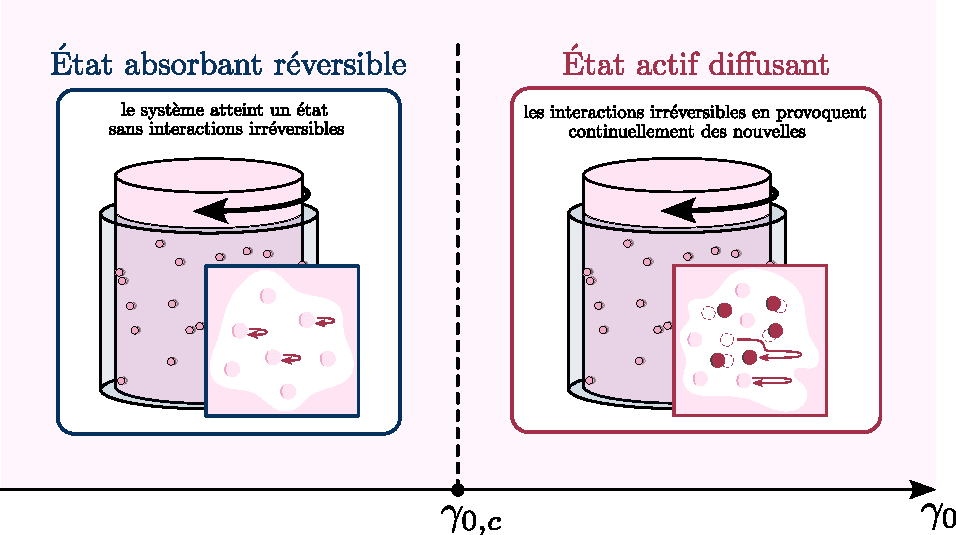
\includegraphics[width=\textwidth]{Chapitre1/Figures/InterpretationCDP/SuspensionsAPT.pdf}
	\caption{Interprétation de la dynamique de la transition de réversibilité comme celle d'une transition de phase absorbante.}
	\label{fig:SuspCDP}
\end{figure}

\subparagraph{}Il y a alors deux possibilités. Dans le premier cas, l'amplitude de cisaillement est suffisamment grande ($\gamma_0 > \gamma_{0,c}$) et la propagation des interactions irréversibles perdure à temps long dans le système, amenant à un coefficient de diffusion stroboscopique non-nul $D_0 >0$. Dans le second cas, l'amplitude de cisaillement globale est trop faible ($\gamma_0 < \gamma_{0,c}$) et le système finit par tomber dans un état réversible où chaque particule suit une orbite stable isolée, amenant à un état stroboscopiquement arrêté $D_0 = 0$.

\subparagraph{}Comme illustré à la \autoref{fig:SuspCDP}, la transition de réversibilité peut donc être comprise comme une transition de phase absorbante dont le paramètre de contrôle est l'amplitude de cisaillement $\gamma_0$ et le paramètre d'ordre le coefficient de diffusion stroboscopique $D_0$. Dans ce système, l'activité est donc directement associée aux déplacements irréversibles des particules, susceptibles de disparaître (via le repositionnement sur une nouvelle orbite stable) ou de se propager (via le repositionnement sur une orbite recoupant une orbite stable), de la même manière que l'activité dans les modèles présentés précédemment. De plus, l'état arrêté dans lequel toutes les particules sont sur une orbite stable est bien un état absorbant puisque la déstabilisation de l'orbite d'une particule ne peut se faire que par l'intersection avec une autre orbite. Ainsi, si toutes les orbites sont stables, elles le resteront pour toujours. Nous pouvons alors définir les mêmes exposants critiques que dans n'importe quelle autre transition de phase absorbante :

\begin{equation}
	D_0 \sim \delta\gamma_0^\beta, \quad \langle \delta D_0^2 \rangle \sim \delta\gamma_0^{-\gamma^\prime},\quad \xi \sim \delta\gamma_0^{-\nu_\perp}, \quad \delta\gamma_0 = \frac{\gamma_0-\gamma_{0,c}}{\gamma_{0,c}}.
\end{equation}

\noindent L'enjeu est alors de connaître la valeur de ces exposants caractérisant cette criticalité.

\subsubsection{Similitudes avec la classe CDP}

\subparagraph{}La classe d'universalité pressentie au premier abord pour la transition de réversibilité est la classe CDP. En effet, nous retrouvons ici un couplage de la propagation de l'activité à celle de la dynamique d'un champ conservé. De fait, les particules, vecteurs de cette propagation dans l'espace, constituent un champ de densité qui, par conservation du nombre de particules (système fermé) est lui-même conservé. De plus, ce système possède un nombre infini d'états absorbants. En effet, tout ensemble d'orbite stable, et il en existe une infinité en espace continu, est un état absorbant. Ainsi, les deux principaux critères de la conjecture de Rossi et. al \cite{rossi_universality_2000} sont respectés. On pourrait donc s'attendre à ce que l'universalité CDP représente cette transition.

\subparagraph{}Afin d'étudier la criticalité de ce système, une approche de modélisation numérique simple a été développée. Celle-ci se concentre uniquement sur la dynamique strobsoscopique du système. Dans ce cadre, comme nous l'expliquerons plus en détail dans le \autoref{chapter:Susp}, le modèle numérique adéquat pour caractériser la transition correspond au ROM que nous avons présenté dans la section précédente. De ce fait, sous cet angle de modélisation, la transition de réversibilité appartient à la classe CDP. Ainsi, en 2D, elle est caractérisée par les exposants critiques $\beta \approx 0.64$ et $\gamma^\prime \approx 0.37$.

\subparagraph{}Toutefois, de notre point de vue, un mécanisme essentiel est perdu dans la simplification de cette modélisation : seules les interactions irréversibles de contact sont prises en compte dans la dynamique du système. Or, dans un système réel, les particules n'interagissent pas seulement par contact direct mais aussi indirectement via le fluide suspendant. Cette simplification est tout sauf anodine puisque, comme nous le discutons dans la partie suivante, la forme pressentie de ces interactions hydrodynamiques est à longue portée. Ceci suggère alors que leur prise en compte est susceptible de modifier significativement la criticalité du système.

\subsubsection{Interactions visqueuses médiées par le fluide}

\label{sec:ref_interac_visc}

\subparagraph{}Dans cette partie nous expliquons brièvement pourquoi nous pensons que le fluide suspendant permet la médiation d'interactions à longue portée entre les particules dans le cadre de la transition de réversibilité, quel que soit le dispositif expérimental considéré. Le raisonnement détaillé est présenté dans l'\annexeref{sec:Annexe_Interactions_Hydro}, nous en présentons simplement ici les conclusions générales dans un souci de concision. Dans le cas de la transition de réversibilité, lorsqu'une particule interagit irréversiblement avec une autre particule au cours d'un cycle, elle quitte son orbite initiale en appliquant une certaine force sur le fluide. Cette force va alors modifier l'écoulement du fluide via les lois régissant sa dynamique et donc affecter le mouvement des particules environnantes. En milieu infini, dans la limite de champ lointain, la force $\mathbf{F}^1(\mathbf{r})=\mathbf{F}^1\delta(\mathbf{r})$ appliquée en $\mathbf{r}$ par une particule $1$ ayant interagi irréversiblement induit une vitesse $\mathbf{v}^2$ sur une particule $2$ située en $\mathbf{r}^\prime$ via la relation linéaire :

\begin{equation}
	v_i (\mathbf{r}^\prime) = \mathcal{G}_{ij}(\mathbf{r} -\mathbf{r}^\prime)F^1_j, \quad \mathcal{G}_{ij}(\mathbf{r}) = \frac{1}{8\pi\eta r}\left( \delta_{ij}+\frac{r_ir_j}{r^2} \right),
\end{equation}

\noindent avec $\mathcal{G}_{ij}$ le tenseur d'Oseen, fonction de Green des équations de Stokes. En pratique cependant, les évènements irréversibles correspondent plutôt à un dipôle de force sur le fluide, représentant le choc des deux particules interagissant. Ainsi, le propagateur d'interaction d'intérêt est plutôt la dérivée de ce tenseur d'Oseen (voir \annexeref{sec:Annexe_Interactions_Hydro}). Celui-ci définit donc une interaction hydrodynamique entre l'évènement irréversibile et les particules environnantes décroissant comme $\sim 1/r^2$ dans le milieu tridimensionnel infini, modélisation adéquate pour décrire le cisaillement de suspensions dans des dispositifs peu confinants.

\subparagraph{}En fait, en se basant sur les principes de conservation de la quantité de mouvement et/ou de la masse dans le système, nous pouvons montrer que dans la grande majorité des dispositifs expérimentaux pertinents pour l'étude de la transition, la forme de l'interaction induite par un monopôle de force reste la même, décrite par :

\begin{equation}
\quad \mathcal{G}_{ij}(\mathbf{r}) \sim \frac{1}{r^\gamma}\left( \delta_{ij}+ C\frac{r_ir_j}{r^2} \right),
\end{equation}

\noindent avec $\gamma$ un entier dépendant du dispositif \cite{diamant_hydrodynamic_2009}. L'interaction entre un évènement irréversible (dipôle de force) et une particule dans la transition de réversibilité décroît donc aussi en loi de puissance comme $\sim 1/r^\alpha$ avec $\alpha = \gamma+1$. Par exemple dans le cas d'un confinement quasi-2D entre deux plaques rigides nous obtenons une décroissance en $\sim 1/r^3$ soit $\alpha = 3$.

\subparagraph{}De manière toute à fait générale, le fluide suspendant permet donc de médier des interactions à longue portée entre les particules. Cette caractéristique n'est pas anodine puisque la conjecture de Rossi et al. \cite{rossi_universality_2000} quant à l'appartenance à la classe CDP suppose implicitement la présence d'interactions à courte portée seulement. La présence d'interactions médiées par le fluide, a priori inévitable, constitue donc un mécanisme de la transition de réversibilité susceptible de rendre sa criticalité différente de celle de la classe CDP. Ce que nous montrons dans la partie suivante est que c'est aussi le cas de la transition vers l'écoulement.

\subsection{Transition vers l'écoulement}

\label{sec:yieldingCDP}

\subparagraph{}En première partie de ce chapitre, nous avons présenté la transition vers l'écoulement des fluides à seuil comme séparant un état coulant d'un état élastique. Pour comprendre plus spécifiquement comment celle-ci peut être appréhendée comme une transition de phase absorbante, il est important de comprendre comment l'écoulement prend place dans la phase active.

\subsubsection{L'écoulement comme une succession de réarrangements}

\subparagraph{}Prenons l'exemple d'un matériau amorphe, comme une mousse, soumis à un cisaillement simple. Lorsque l'on applique une certaine contrainte de cisaillement $\Sigma$ à ce système, celle-ci se voit supportée par les différentes régions du matériau sous forme de contrainte locale $\sigma$. Dans la limite où cette contrainte locale est suffisamment faible, la région associée la supporte en opérant une déformation élastique. Cependant, dès lors que cette contrainte locale dépasse un certain seuil $\sigma_Y$, propre à chaque région, la région associée se déforme plastiquement et irréversiblement. Cette déformation plastique permet alors de relaxer la trop forte contrainte locale et, par conservation de la contrainte appliquée, de la redistribuer aux autres régions du matériau \cite{nicolas_deformation_2018}. 

\subparagraph{}Dans le cas des mousses, les réarrangements plastiques permettant la relaxation de la contrainte locale prennent une forme bien spécifique : les évènements dits T1 \cite{princen_rheology_1986}. Au cours d'un tel évènement, un groupe de quatre bulles (correspondant à une région locale précédemment mentionnée) opère un changement topologique par changement de voisins. Ce processus géométrique de relaxation local de la contrainte est illustré à la \autoref{fig:yieldingchapo}-(a) via les images tirées de \cite{dollet_rheology_2014}. Ce type de réarrangement plastique caractéristique est retrouvé dans l'écoulement d'autres systèmes amorphes comme les émulsions ou les verres métalliques, impliquant dans ce cas un plus grand nombre d'entités microscopiques \cite{nicolas_deformation_2018}. 

\subparagraph{}En redistribuant la contrainte locale relaxée, une région se réarrangeant plastiquement est capable d'induire le dépassement du seuil de contrainte local dans une autre région du matériau. Celle-ci va alors à son tour se réarranger plastiquement, redistribuer son surplus de contrainte locale et déclencher de nouveaux évènements dans le système. Mises à la suite les unes des autres, ces déformations plastiques locales créent alors un écoulement plastique macroscopique global via une dynamique collective.

\subparagraph{}Il y a alors deux possibilités. Dans le premier cas, la contrainte globale appliquée au système $\Sigma$ est trop faible ($\Sigma<\Sigma_c$) et le système finit par tomber dans un état où toutes les régions du matériau sont capables de soutenir la contrainte locale élastiquement ($\sigma < \sigma_Y$). Le matériau ne coule donc pas, on observe un taux de cisaillement nul $\dot{\gamma} = 0$. Dans le second cas, la contrainte globale est suffisamment grande ($\Sigma>\Sigma_c$) pour que, à temps long, le système soit toujours traversé par des réarrangements plastiques locaux. Dans l'état stationnaire, le matériau s'écoule et on mesure un taux de cisaillement non-nul $\dot{\gamma}>0$. Il est important de noter que la dynamique collective complexe à l’œuvre fait que la contrainte seuil globale $\Sigma_c$ ne peut pas être trivialement déduite des contraintes seuil locales $\sigma_Y$.

\begin{figure}[h]
	\centering
	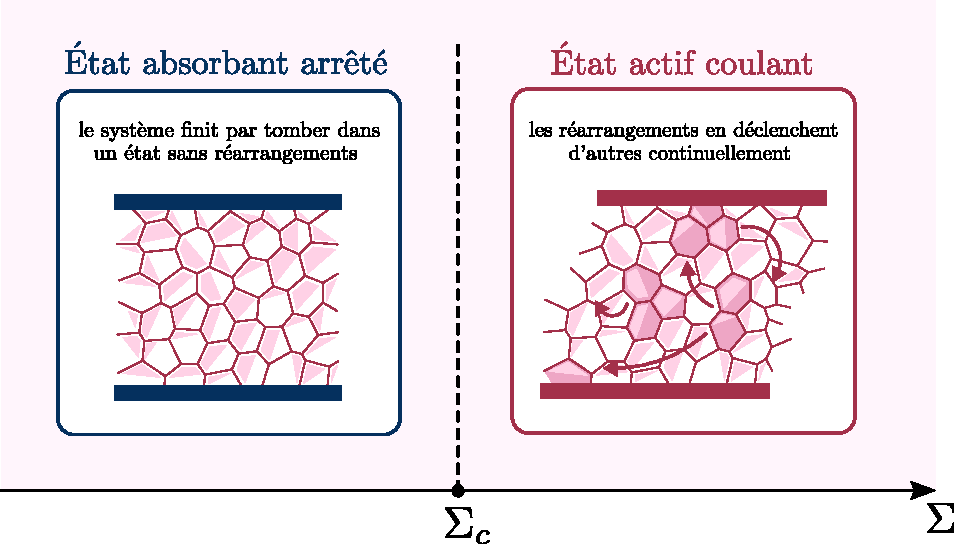
\includegraphics[width=\textwidth]{Chapitre1/Figures/InterpretationCDP/YieldingAPT.pdf}
	\caption{Interprétation de la dynamique de l'écoulement des fluides à seuil comme celle d'une transition de phase absorbante.}
	\label{fig:YieldingCDP}
\end{figure}

\subparagraph{}Comme illustré à la \autoref{fig:YieldingCDP}, la transition vers l'écoulement peut donc être comprise comme une transition de phase absorbante dont le paramètre de contrôle est la contrainte de cisaillement $\Sigma$ et le paramètre d'ordre le taux de cisaillement $\dot{\gamma}$. Dans ce système, l'activité est donc directement associée à la déformation plastique locale du matériau qui est susceptible de s'estomper (via la relaxation de la contrainte locale) comme de se propager (via la redistribution de contrainte), de la même façon que dans les modèles précédemment évoqués dans ce chapitre. Par ailleurs, l'état arrêté représenté par $\dot{\gamma} = 0$ est bien un état absorbant de la dynamique puisque, à $\Sigma$ fixée, un réarrangement plastique ne peut être provoqué que par la redistribution de contrainte engendrée par un réarrangement précédent. De cette façon, on peut définir les mêmes exposants critiques que dans le cadre de n'importe quelle autre transition de phase absorbante :

\begin{equation}
	\dot{\gamma} \sim \delta\Sigma^\beta,\quad \langle\Delta\dot{\gamma}^2\rangle \sim \delta\Sigma^{-\gamma^\prime}, \quad \xi \sim \delta\Sigma^{-\nu_\perp}, \quad \delta\Sigma = \frac{\Sigma-\Sigma_c}{\Sigma_c}.
\end{equation}

\subparagraph{}Il ne va pas sans remarquer que la phénoménologie décrite de la transition vers l'écoulement ressemble fortement à celle de la transition de dépiégeage. On peut en effet faire une analogie directe entre la contrainte globale de cisaillement $\Sigma$ et la force extérieure $f$ de la transition de dépiégeage, et entre le taux de cisaillement $\dot{\gamma}$ et la vitesse de l'interface $v$ dans la transition de dépiégeage. D'ailleurs, plusieurs études se sont concentrées sur la comparaison de ces deux phénomènes \cite{lin_scaling_2014, ferrero_elastic_2019, tyukodi_depinning_2016}. Dans cette optique, on pourrait s'attendre naturellement à ce que la transition vers l'écoulement soit aussi représentée par la classe CDP.

\subsubsection{Similitudes avec la classe CDP}

\subparagraph{}La transition vers l'écoulement semble en effet réunir la plupart des conditions pour l'appartenance à l'universalité CDP. De fait, celle-ci présente une dynamique d'activité couplée à celle d'un champ conservé non-diffusif : le champ de contrainte locale. Par ailleurs, cette transition possède une infinité d'états absorbants. En effet, n'importe quel état du système possédant un champ de contrainte local vérifiant $\sigma < \sigma_Y$ en tout point du matériau est un état absorbant. Les deux critères de la conjecture de Rossi et al. \cite{rossi_universality_2000} sont donc bien vérifiés.

\subparagraph{}Cependant, comme pour la transition de réversibilité, la transition vers l'écoulement fait intervenir des interactions à longue portée, contredisant la condition de courte portée implicitement inscrite dans la conjecture de Rossi et al \cite{rossi_universality_2000}. En effet, nous montrons dans la partie suivante que le milieu élastique dans lequel prennent place les réarrangements plastiques permet de redistribuer la contrainte relaxée à longue portée.

\subsubsection{Interactions élastiques médiées par le solide}

\label{sec:ref_interac_elast}

\subparagraph{}L'effet d'un réarrangement plastique sur le milieu peut être compris dans le cadre de l'élasticité linéaire. Dans cette partie, nous présentons les conclusions du raisonnement mené dans l'\annexeref{sec:Annexe_Eshelby}, permettant de déterminer la modification de contrainte induite par un réarrangement plastique dans le système. Dans un matériau élastique isotrope et incompressible de module de cisaillement $\mu$, une déformation plastique représentée par le tenseur $\epsilon_{ij}^\text{pl}(\mathbf{r})$ entraîne une modification du tenseur des contraintes $\sigma_{ij}(\mathbf{r})$ décrite par la relation linéaire :

\begin{equation}
	\sigma_{ij}(\mathbf{r}) = \int\mathrm{d}\mathbf{r}^\prime~ \mathcal{G}_{ijkl}(\mathbf{r}-\mathbf{r}^\prime)\epsilon^\text{pl}_{kl}(\mathbf{r}^\prime),
\end{equation}

\noindent avec $\mathcal{G}_{ijkl}$ un propagateur dont la forme générale est donnée en annexe.

\subparagraph{}Afin d'obtenir une expression de la modification du champ de contrainte suite à un réarrangement plastique, nous faisons l'hypothèse que celui-ci possède la même symétrie que le forçage, que nous prenons comme un cisaillement simple dans la direction $\hat{\mathbf{e}}_x$. En considérant l'évènement comme ayant lieu en $\mathbf{r}^\prime = 0$, on a alors en 2D : $\epsilon_{xy}^\text{pl}(\mathbf{r}^\prime) = \epsilon_{yx}^\text{pl}(\mathbf{r}^\prime) = \epsilon^\text{pl}\delta(\mathbf{r}^\prime)$ et $\epsilon_{xx}^\text{pl}(\mathbf{r}^\prime) = \epsilon_{yy}^\text{pl}(\mathbf{r}^\prime) = 0$. Via cette modélisation, la modification de la contrainte locale de cisaillement\footnote{Des expressions similaires peuvent être obtenues pour les composantes $\sigma_{xx}$ et $\sigma_{yy}$ du tenseur des contraintes. Toutefois, on se concentrera ici seulement sur la contrainte locale de cisaillement $\sigma_{xy}$.} dans le matériau est donnée par :

\begin{equation}
	\sigma_{xy}(\mathbf{r})= \sigma_{yx}(\mathbf{r}) = 2\mu \mathcal{G}(\mathbf{r}) \epsilon^\text{pl}, \quad \mathcal{G}(\mathbf{r}) = \frac{\cos (4\theta)}{\pi r^2}.
	\label{eq:Eshelby}
\end{equation}

\subparagraph{}On appelle alors le propagateur $\mathcal{G}$ propagateur d'Eshelby\footnote{Sa dénomination revient à la personne l'ayant calculé en premier \cite{eshelby_determination_1997}.}, dont la forme correspond à la modification de contrainte à l'issue d'un unique réarrangement plastique localisé. La redistribution de contrainte opérée lors d'un tel évènement est donc effectivement à longue portée, décroissant comme $\sim 1/r^2$ en 2D.

\paragraph{Forme et observations expérimentales}

\subparagraph{}Sur la \autoref{fig:EshelbyExp}-(a), nous représentons la redistribution de la contrainte de cisaillement locale suite à un réarrangement plastique. Comme on peut le remarquer, en plus d'être à longue portée, la redistribution est fortement anisotrope. Plus particulièrement, le signe de celle-ci dépend de la direction considérée : la redistribution est positive dans les directions principales du cisaillement $\hat{\mathbf{e}}_x$ et $\hat{\mathbf{e}}_y$ et négative dans les directions intermédiaires. En d'autres termes, un réarrangement plastique d'une région dans le milieu élastique déstabilise aussi bien qu'il ne stabilise les autres régions. Par ce mécanisme, la plasticité dans le milieu favorise donc la propagation de l'activité en même temps qu'elle l'inhibe (une redistribution de contrainte négative défavorise le déclenchement d'un nouveau réarrangement plastique).

\begin{figure}[h]
	\centering
	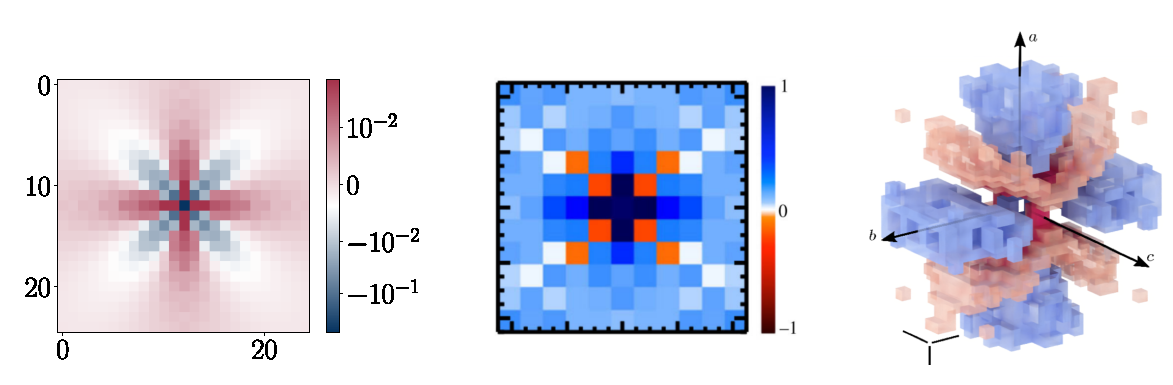
\includegraphics[width=\textwidth]{Chapitre1/Figures/InterpretationCDP/EshelbyExp.pdf}
	\caption{Anisotropie de la redistribution de contrainte après un réarrangement plastique (les unités spécifiques n'ont pas d'importance). (a) Représentation en 2D du propagateur d'Eshelby défini par l'\autoref{eq:Eshelby}. (b) Redistribution de contrainte suite à un réarrangement plastique mesurée dans \cite{desmond_measurement_2015}. (c) Idem dans \cite{schott_multiscale_2024}, les zones rouges représentent des redistributions positives et les zones bleues des redistributions négatives.}
	\label{fig:EshelbyExp}
\end{figure}

\subparagraph{}La redistribution de la contrainte suite à un tel évènement a été mesurée en conditions réelles dans différents systèmes, confirmant la forme prédite par la théorie continue \cite{desmond_measurement_2015, schott_multiscale_2024, jensen_local_2014}. Par exemple, dans \cite{schott_multiscale_2024}, les auteurs ont mesuré la redistribution de contrainte dans une mousse après un évènement T1 et ont pu mettre en évidence la forme quadrupolaire caractéristique du propagateur d'Eshelby. D'autre part, via des simulations de dynamique moléculaire, la topologie et la portée de l'interaction d'Eshelby s'est aussi vue confirmée dans différents systèmes \cite{kabla_local_2003, maloney_amorphous_2006, tanguy_plastic_2006}. Cette forme simple de l'interaction permet alors d'encoder le mécanisme d'écoulement des fluides à seuil dans des modèles mésoscopiques que nous présenterons au \autoref{chapter:yielding}.

\subparagraph{}De la même façon que dans le cas des suspensions, les dispositifs expérimentaux étudiés peuvent agir significativement sur la portée des interactions. Si l'on considère par exemple un écoulement quasi-2D entre deux plaques rigides, celui-ci implique une redistribution de contrainte suite à un évènement plastique décroissant comme $\sim 1/r^4$ à grande distance (voir \autoref{sec:lambda_picard}). Ainsi, comme dans le cas des suspensions, le caractère de longue portée des interactions médiées est génériquement présent.

\subparagraph{}In fine, il semble donc aussi que la transition vers l'écoulement des fluides à seuil peut être comprise dans le cadre CDP avec la présence additionnelle d'interactions à longue portée.

\section{Atypicité des transitions étudiées}

\subparagraph{}D'après les éléments soulevés dans la section précédente, les transitions de réversibilité et d'écoulement semblent correspondre au cadre de description CDP en présence d'interactions à longue portée. Dans le cadre d'étude des transitions de phase continues, l'influence des interactions à longue portée sur le comportement critique peut être compris dans un cadre générique. Dans cette section, nous montrons via des mesures pré-existantes que les transitions que nous proposons d'étudier dans cet ouvrage ne peuvent en fait pas être rapportées à ce cadre. Nous proposons alors une explication à cette divergence via la nature des interactions qu'elles mettent en place. Celles-ci définissent en effet un mécanisme de propagation de l'activité original, échappant au cadre théorique habituel.

\subsection{Incompatibilité avec le cadre générique de la longue portée}

\subsubsection{Attendu générique de l'influence d'interactions à longue portée}

\subparagraph{}Dans un système présentant des interactions à longue portée, décroissant comme ${\sim 1/r^\alpha}$, tous les agents microscopiques sont liés. Ce lien est d'autant plus fort que la portée de l'interaction est grande (i.e. $\alpha$ petit). Dans la limite où cette portée est infinie, tous les agents interagissent de manière équivalente entre eux, détruisant ainsi la notion d'espace dans le système. De ce fait, son comportement équivaut à celui du champ moyen associé. \`A l'opposé de ce spectre, dans la limite où cette portée est infiniment faible, l'interaction non-locale n'est significative que dans le voisinage direct de chaque agent. Ainsi, ce cas se rapporte à la présence d'interactions locales uniquement.

\subparagraph{}Cette phénoménologie trouve écho dans les phénomènes critiques. Lorsque l'on généralise l'interaction locale sous-jacente d'un phénomène critique au cas de longue portée, décrit par un exposant $\alpha$, le comportement critique présente deux cas limites. Dans la limite de grande portée, le comportement critique retrouvé est celui du champ moyen, décrit par des exposants critiques triviaux. \`A l'inverse, dans la limite de courte portée, les exposants critiques décrivant le système prennent leur valeur non-triviale de dimension finie. Dans un système présentant des interactions caractérisées par un exposant $\alpha$ arbitraire, on s'attendra donc à trouver une criticalité encadrée par son équivalent de courte portée et le champ moyen associé.

\subparagraph{}Par exemple, dans le cas de nos deux transitions d'intérêt, la classe a priori adéquate pour décrire le comportement à courte portée est la classe CDP. Ainsi, avec la présence additionnelle d'interactions à longue portée, on peut s'attendre à mesurer des exposants critiques compris entre ceux donnés par la criticalité CDP en dimension finie et ceux donnés par la criticalité CDP en champ moyen. D'après les valeurs connues de ces deux limites que nous avons répertoriées au \autoref{tab:expocrit_DPCDP}, on s'attendrait par exemple à mesurer en 2D un exposant $\beta$ encadré comme $0.64 < \beta < 1$ et un exposant $\gamma^\prime$ encadré comme $0 < \gamma^\prime < 0.37$.

\subparagraph{}Dans la partie suivante, nous montrons que les mesures réalisées précédemment sur des systèmes représentant ces transitions contredisent cette attente naturelle.

\subsubsection{Contradiction du cadre générique par les transitions de réversibilité et d'écoulement}

\paragraph{Transition de réversibilité}

\subparagraph{}Dans une étude menée par Mari et. al \cite{mari_absorbing_2022}, les auteurs ont proposé de pallier à l'absence des interactions hydrodynamiques dans les simulations numériques stroboscopiques pré-existantes. Pour ce faire, en reprenant le cadre de modélisation offert par le ROM, les auteurs ont explicitement intégré l'effet de ces interactions en les représentant par une diffusion effective des particules. Celle-ci est décrite par un coefficient de diffusion proportionnel au nombre de particules actives (i.e. subissant une interaction de contact irréversible à un instant $t$) dans le système. Cela équivaut alors en quelque sorte à considérer les interactions médiées dans une approche de champ moyen, c'est-à-dire de portée infinie\footnote{La philosophie derrière cette modélisation sera présentée plus en détail au \autoref{chapter:Susp}.} ($\alpha = 0$). 

\subparagraph{}Ce faisant, les auteurs ont étudié le comportement critique du système en 2D et mesuré les exposants critiques $\beta$ et $\gamma^\prime$ associés, trouvant les valeurs :

\begin{equation}
	\beta \approx 1.85 \quad \gamma^\prime \approx -1.2.
\end{equation}

\noindent Ces valeurs sont alors en contradiction avec l'effet générique des interactions à longue portée sur la classe CDP, puisqu'elles ne sont pas encadrées par les limites de champ moyen et de courte portée associées. Notamment, elles décrivent une évolution convexe du paramètre d'ordre avec la distance au point critique ($\beta >1$), là où la criticalité CDP généralisée au cas d'interactions à longue portée décrit une évolution concave, voire linéaire ($\beta = 1$). Même si l'implémentation de ces interactions peut être discutée (dans un système réel, nous avons montré que leur portée était caractérisée par $\alpha > 0$), leur intégration dans le modèle semble exclure la transition de l'attendu générique.


\begin{figure}[h]
	\centering
	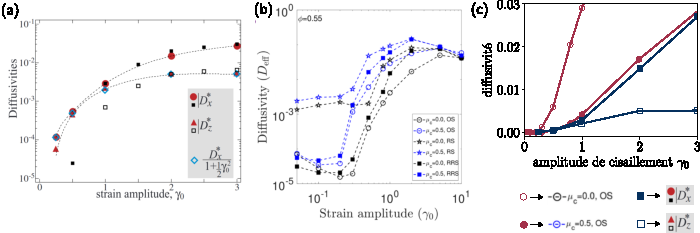
\includegraphics[width=\textwidth]{Chapitre1/Figures/LongRange/ExpShear.pdf}
	\caption{Caractérisation de la transition de réversibilité dans les suspensions cisaillées cycliquement dans des études de dynamique moléculaire. Évolution de la diffusivité stroboscopique avec l'amplitude de cisaillement dans l'étude \cite{metzger_irreversibility_2010} (a) et \cite{agrawal_dense_2024} (b). (c) Représentation lin-lin de certaines courbes tirées de (a) et (b), spécifiées dans la légende.}
	\label{fig:ShearedExp}
\end{figure}

\subparagraph{}Si l'on regarde du côté des expériences (voir \autoref{fig:suspchapo}-(b)) ou des simulations plus réalistes de dynamique moléculaire, les mesures proposées sur ces systèmes ne semblent par ailleurs pas vraiment contredire cette observation. En effet, sur la \autoref{fig:ShearedExp}-(c) où nous avons reproduit les résultats des études \cite{metzger_irreversibility_2010, agrawal_dense_2024}, il n'apparaît pas clairement que l'évolution du paramètre d'ordre soit concave et semble même convexe. 

\subparagraph{}Ces éléments suggèrent alors que la transition de réversibilité pourrait ne pas être appréhendée via l'extension à longue portée générique de la classe CDP. Dans la sous-section suivante, nous montrons qu'il en est de même pour la transition vers l'écoulement.

\paragraph{Transition vers l'écoulement}

\subparagraph{}La criticalité de la transition vers l'écoulement a été déjà étudiée via des modèles mésoscopiques numériques en deux dimensions que nous présenterons au \autoref{chapter:yielding}\cite{lin_scaling_2014, liu_driving_2016, ferrero_criticality_2019, picard_slow_2005}. Dans les travaux associés, l'exposant $\beta$ a été mesuré à plusieurs reprises comme $\beta\approx 1.5$, montrant ainsi à nouveau une évolution convexe du paramètre d'ordre avec la distance au point critique.

\subparagraph{}Ces mesures sont en accord qualitatif avec de nombreuses expériences réalisées sur les fluides à seuil. Dans ce domaine d'étude, il est d'usage de modéliser la courbe d'écoulement $\dot{\gamma} = f(\Sigma)$ du système par la loi d'Herschel-Bulkley :

\begin{equation}
	\Sigma = \Sigma_c + k\dot{\gamma}^n, \quad k > 0,
\end{equation}

\noindent avec $n$ l'exposant d'Hershel-Bulkley, directement associé à l'exposant $\beta$ des phénomènes critiques via $n=1/\beta$. De nombreux travaux, menés sur différents systèmes amorphes, ont déterminé des exposants $n<1$ soit $\beta > 1$, correspondant à une transition vers l'écoulement convexe, comme dans le cas des modèles mésoscopiques \cite{nicolas_deformation_2018}.

\subparagraph{}Ces éléments suggèrent donc que la transition vers l'écoulement, comme la transition de réversibilité, ne correspond pas à l'attente naturelle de l'extension à longue portée de la classe CDP. De ce point de vue, ces deux transitions présentent un point commun très fort, qui motive leur étude simultanée. Cette étude est en fait d'autant plus intéressante qu'un indice apparent semble par ailleurs rapprocher ces deux transitions tout en les éloignant du cadre générique : dans ces deux systèmes, les interactions à longue portée induisent un mécanisme de propagation de l'activité original.

\subsection{Des interactions à longue portée de nature différente}

\subsubsection{La longue portée comme transport dans le cadre d'interprétation générique}

\subparagraph{}En fait, comme nous le détaillerons dans le \autoref{chapter:TransportLP}, dans le cadre générique d'évolution de la criticalité CDP avec les interactions à longue portée, celles-ci sont représentées par un transport à longue portée de la quantité conservée induit localement par l'activité.

\subparagraph{}Dans le cadre des modèles de particules comme le modèle Manna ou le ROM, cela revient à considérer que les particules actives font des sauts $\mathbf{r}^\prime$ distribués selon $P(\mathbf{r}^\prime)\sim 1/|\mathbf{r}^{\prime}|^{\alpha}$, et non plus uniquement dans leur voisinage direct. Dans cette approche, les interactions à longue portée représentent donc un transport de masse à longue portée induit localement par l'activité.

\subparagraph{}Dans le cas de la transition de dépiégeage, nous avions associé la redistribution de masse à la redistribution de force élastique. Ainsi, l'extension à longue portée de ce phénomène correspond dans ce cas à des interactions élastiques à longue portée. Le propagateur qui redistribue cette force élastique est alors le pendant direct de la distribution de probabilité des sauts dans les modèles de particules. On peut donc voir dans la transition de dépiégeage à longue portée un transport de la force élastique à longue portée induit localement par l'activité. C'est en fait un cas d'étude qui a concentré de nombreux travaux car certains problèmes de dépiégeage présentent de l'élasticité à longue portée (voir \annexeref{app:exp_depinning}).


\subparagraph{}Ce que nous montrons dans cette sous-section, c'est que les interactions à longue portée médiées par le milieu dans les transitions de réversibilité et d'écoulement ne peuvent pas vraiment être comprises comme un transport à longue portée de la quantité conservée induit localement par l'activité, ou en tous cas pas complètement.

\begin{figure}[h]
	\centering
	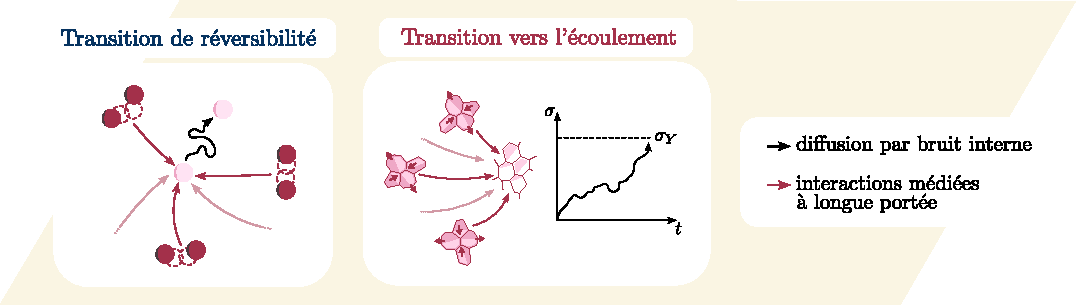
\includegraphics[width=\textwidth]{Chapitre1/Figures/Pb/bruit.pdf}
	\caption{Nouveaux mécanismes de création d'activité induits par les interactions à longue portée dans la transition de réversibilité et la transition vers l'écoulement.}
	\label{fig:bruit}
\end{figure}

\subsubsection{La longue portée comme source de diffusion dans les transitions de réversibilité et d'écoulement}

\paragraph{Transition de réversibilité}

\subparagraph{}Dans le cas de la transition de réversibilité, les interactions hydrodynamiques provoquent des petits déplacements des particules dans tout le milieu suite à un évènement irréversible. Ainsi, ce n'est pas la particule à l'origine de l'interaction irréversible qui est transportée à longue portée, mais plutôt l'influence de l'activité sur les particules qui est à longue portée. Dans ce cas, la longue portée ne prend pas la forme d'un transport mais plutôt d'un bruit interne : chaque particule est soumise à des petits déplacements induits à longue portée par l'activité dans le système. Un nouveau mécanisme potentiel de création d'activité prend place : via l'influence de ce bruit interne, l'orbite stable associée à une particule passive peut se déformer progressivement jusqu'à rencontrer une autre orbite stable et ainsi créer un évènement irréversible. En d'autres termes, la création d'activité peut être approchée par une sorte de diffusion (et non plus par un déplacement fini issu d'un évènement irréversible précédent) induite de manière non-locale.

\paragraph{Transition vers l'écoulement}

\subparagraph{}Comme nous l'avons mentionné à la \autoref{sec:yieldingCDP}, la transition vers l'écoulement est très proche de celle du dépiégeage. De la même façon que l'on peut voir la redistribution de force élastique dans le dépiégeage comme un transport induit localement par l'activité, on peut appréhender une partie de la redistribution de contrainte dans la transition vers l'écoulement comme tel. Lors du réarrangement plastique d'une région, la contrainte locale de celle-ci est relaxée et transmise aux autres régions du matériau. Toutefois, l'effet complet de la redistribution ne peut pas être appréhendé comme tel. En effet, comme nous l'avons mentionné à la \autoref{sec:yieldingCDP}, le propagateur d'Eshelby est de signe alterné. Ainsi, à la différence du propagateur élastique associé au dépiégeage qui est toujours positif, il ne peut pas être le pendant direct de la distribution de probabilité associée au transport de masse dans les modèles de particules. \`A la place, la propriété de signe alterné montre qu'une partie de l'interaction peut être comprise comme un bruit mécanique, qui peut autant stabiliser que déstabiliser une région du matériau. Cette interprétation n'est d'ailleurs pas nouvelle dans le cadre de cette transition \cite{lin_mean-field_2016, ferrero_criticality_2019}. Ainsi, en plus du mécanisme de transport induit localement par l'activité qui tend à déstabiliser globalement le matériau, un mécanisme de diffusion induite non-localement des contraintes locales vers les contraintes seuils locales prend place (voir \autoref{fig:bruit}). De la même manière que dans la transition de réversibilité, on a donc un mécanisme de création de l'activité par diffusion induite de manière non-locale.

\subparagraph{}Finalement, dans ces deux transitions présentant un comportement critique non conventionnel, nous retrouvons un mécanisme de création de l'activité par diffusion issu des interactions à longue portée. Nous pensons alors que c'est ce mécanisme qui permet d'expliquer les spécificités associées à la transition de réversibilité dans les suspensions cisaillées cycliquement et à la transition vers l'écoulement des fluides à seuil, en contradiction avec l'attente naturelle de l'effet d'interactions à longue portée sur un phénomène critique. \`A partir de ce point plusieurs questions se posent, lesquelles constitueront le fil conducteur de cette thèse.

\section{Problématisation}

\subsection{Questions guidant ce travail}

\paragraph{Quelle criticalité caractérise les transitions de réversibilité et d'écoulement ?}

\subparagraph{}Le premier axe de recherche autour duquel s'articule ce travail correspond à la caractérisation des deux transitions. Nous nous demanderons notamment quelles sont les valeurs prises par les exposants critiques dans le cas d'interactions à longue portée réalistes, i.e. réalisables en conditions expérimentales. Plusieurs questions concernant cette caractérisation découlent de l'étude menée par Mari et al. \cite{mari_absorbing_2022} sur la transition de réversibilité avec portée infinie des interactions médiées par le milieu. 

\subparagraph{}Nous nous demanderons d'abord si les spécificités non-conventionnelles révélées par cette étude sont toujours présentes dans un système présentant une transition de réversibilité avec des interactions décroissant en loi de puissance avec la distance ($\alpha > 0$). Notamment, nous chercherons à savoir si la transition reste dans ce cas convexe ($\beta >1$) et avec des fluctuations qui s'annulent à l'approche du point critique ($\gamma^\prime < 0$) comme observé par Mari et al. \cite{mari_absorbing_2022}. Par ailleurs, dans cette étude de portée infinie, la double non-conventionnalité $\beta >1$ et $\gamma^\prime < 0$ avait été rationalisée par la relation d'hyperscaling $2\beta + \gamma^\prime = \nu_\perp D$, qui justifie une valeur anormalement faible de $\gamma^\prime$ par une valeur anormalement grande de $\beta$. Les caractérisations précédentes de la transition vers l'écoulement révélant un exposant $\beta >1$, nous nous demanderons alors si, vue comme une transition de phase absorbante, celle-ci présente aussi des fluctuations d'activité qui s'annulent à l'approche du point critique.

\subparagraph{}Mari et al. ont par ailleurs montré que la propriété d'hyperunformité était effacée par l'ajout des interactions hydrodynamiques de portée infinie. Nous nous demanderons alors si cette perte d'hyperuniformité est aussi retrouvée dans les cas de portées réalistes de l'interaction. Par analogie, nous transposerons cette question dans le cas de la transition vers l'écoulement : le système présente-t-il une forme d'hyperuniformité en présence des interactions élastiques d'Eshelby à longue portée ?

\subparagraph{}Enfin, nous nous intéresserons à la forme prise par les dynamiques d'avalanche proche du point critique dans ces deux systèmes.

\paragraph{Quelle est l'influence de la portée des interactions médiées sur la criticalité de ces systèmes ?}

\subparagraph{}Dans le \autoref{chapter:TransportLP}, nous présenterons plus en détail le cadre générique d'appréhension des interactions à longue portée, comprises alors comme un transport à longue portée de la quantité conservée induit localement par l'activité, dans un système appartenant à la classe CDP. Celui-ci montre en fait une évolution de la criticalité bien définie en fonction de la valeur de $\alpha$.

\subparagraph{}Or, nous avons montré que les transitions de réversibilité et d'écoulement ne semblent pas pouvoir être décrites dans ce cadre. Dès lors, le rôle de la longue portée des interactions dans ces systèmes n'est pas évident. Nous chercherons à comprendre de manière systématique l'influence de la portée sur les différents aspects de la criticalité de ces systèmes, i.e. à déterminer comment évoluent les exposants critiques caractérisant l'état stationnaire du système, ceux caractérisant son hyperuniformité et ceux caractérisant sa dynamique d'avalanche en fonction de l'exposant de portée $\alpha$.

\subparagraph{}Nous chercherons alors à comparer ces évolutions avec celles du cadre générique, afin de comprendre dans quelle mesure cette nature différente des interactions rend le cadre d'appréhension usuel inadéquat.

\paragraph{Peut-on comprendre ces systèmes similaires dans un cadre de description commun ?}

\subparagraph{}Le troisième axe d'étude consiste à comprendre la transition de réversibilité et d'écoulement dans un cadre commun. Notamment nous nous interrogerons sur la possibilité d'une description champ moyen permettant de rendre compte des observations faites sur les dynamiques en dimension finie, via la prise en compte du nouveau mécanisme de création proposé par les interactions médiées à longue portée. La mise en place de ce cadre pourrait alors aider à mettre en évidence les similarités et les différences éventuelles entre ces deux phénomènes. Aussi, nous nous interrogerons sur la possibilité d'une description continue, à la manière des équations de champ dans la théorie CDP et son extension à longue portée, pour décrire la dynamique de ces systèmes en toute dimension.

\subsection{Déroulé du manuscrit}

\subparagraph{}Pour répondre à toutes les questions révélées par ce chapitre, nous organiserons ce manuscrit comme suit :

\subparagraph{}Dans le \autoref{chapter:TransportLP}, nous caractériserons quantitativement le cadre générique d'appréhension de la longue portée en 2D pour pouvoir mener convenablement, par contraste, l'étude des transitions de réversibilité et d'écoulement dans les chapitres suivants. Pour ce faire, nous généraliserons les modèles Manna et ROM dans le cas d'un transport à longue portée et caractériserons l'évolution des exposants critiques et des propriétés d'hyperuniformité en fonction de la portée de la redistribution de masse. 

\subparagraph{}Dans le \autoref{chapter:Susp}, nous nous concentrerons sur la transition de réversibilité dans les suspensions cisaillées cycliquement. En généralisant le modèle numérique initialement proposé par Mari et al. \cite{mari_absorbing_2022}, nous étudierons la criticalité du système associée à différentes portées des interactions médiées. Cette caractérisation se fera via la détermination des exposants critiques et l'étude des propriétés d'hyperuniformité et des statistiques d'avalanches. Ensuite, nous proposerons un modèle champ moyen permettant de rendre compte des spécificités de la transition via la compréhension du mécanisme de diffusion induit par les interactions médiées à longue portée. Nous comparerons enfin les prédictions de ce modèle avec les résultats obtenus en dimension finie afin de mettre en évidence les sources de complexité dans la dynamique réelle.

\subparagraph{}Dans le \autoref{chapter:yielding}, nous nous concentrerons sur la transition vers l'écoulement des fluides à seuil. Nous proposerons tout d'abord une étude détaillée de la transition en présence d'interactions élastiques d'Eshelby, via l'utilisation d'un modèle mésoscopique numérique. Ensuite, nous mettrons en évidence deux ingrédients susceptibles d'expliquer les spécificités de la criticalité associée : celui déjà évoqué concernant la nature spécifique des interactions à longue portée, et une symétrie particulière retrouvée dans le propagateur de redistribution. Puis, nous procéderons à une généralisation de notre modèle pour étudier différentes portées d'interactions afin de comprendre l'influence de ces dernières sur le comportement critique. Comme pour les modèles précédents, cette caractérisation portera sur l'évolution des exposants critiques, des propriétés d'hyperuniformité et de la dynamique d'avalanche.

\subparagraph{}Enfin, dans un dernier chapitre, nous mettrons face à face les résultats obtenus dans les deux chapitres précédents. Cela nous permettra de tisser une analogie directe entre la transition de réversibilité dans les suspensions cisaillées cycliquement et la transition vers l'écoulement des fluides à seuil. Nous discuterons alors de l'application à la transition vers l'écoulement du cadre théorique présenté au \autoref{chapter:Susp} pour la transition de réversibilité. Cette analyse permettra de souligner les points communs et les différences entre les deux systèmes et d'en fournir une image globale, montrant l'utilité d'une telle étude comparée.